\documentclass[%
openright%
]{settings/UUThesisTemplate}
%%%%%%%%%%%%%%%%%%%%%%%%%%%%%%%%%%%%%%%%%%%

\newcommand{\bjcom}[1]{\textcolor{blue}{\sl [#1]}}
\newcommand{\bjfix}[2]{{\sl [\textcolor{red}{#1} -> \textcolor{green}{#2}]}}
\newcommand{\bjcor}[1]{{\sl [\textcolor{red}{should be} \textcolor{green}{``#1''}]}}


\newcommand{\authorSurname}{Haziza}
\newcommand{\authorFirstName}{Frédéric}
\newcommand{\authorFirstInitial}{F}
\newcommand{\authorEmail}{daz@it.uu.se}
\newcommand{\dissertationTitle}{Few is Just Enough!}
\newcommand{\dissertationSubtitle}{Small Model Theorem for Parameterized Verification and Shape Analysis}

\keywords{program verification, model checking, parameterized systems, infinite-state systems, reachability, approximation, safety, tree systems, shape analysis, small model properties, view abstraction, monotonic abstraction} % comma-separated


\newcommand{\disputationLanguage}{English}
\newcommand{\numberOfPages}{123} % The page number of the last page
\newcommand{\placeOfDisputation}{ITC 2446, Polacksbacken} % Place of disputation. Ex: Siegbansalen, Ångström Laboratory
\newcommand{\dateOfDisputation}{Wednesday, November 18, 2015} % Date of disputation (Day, Month, Year) Ex: Friday, February 1, 2008
\newcommand{\timeOfDisputation}{13:15} % Time of disputation (Swedish time format). Ex 13:15
\newcommand{\placeOfPublication}{Uppsala} % The place of publication
\newcommand{\yearOfPublication}{2015}

\newcommand{\department}{Division of Computer Systems\\Department of Information Technology} % Name of your department
\newcommand{\departmentaddress}{Lägerhyddsvägen 2, 752 37 Uppsala, Sweden} % Address of your department


\titlepagelogo{img/UU_logo_sv_42.pdf}
\title{{\TitleFont Few\ \ is~Just~Enough!}}
\subtitle{\texorpdfstring{Small Model Theorem %for
    $\left\{\begin{array}{l}\text{Parameterized Verification} \\ \text{Shape Analysis}\end{array}\right.$}{Small Model Theorem for Parameterized Verification and Shape Analysis}}

\ifunderprogress\else%%%%%%%%%%%%%%%%%%%%%%%%%%%%%%
% Abstract redefinition
\abstractdummy{\begin{abstract}%%
%This doctoral thesis considers the automatic verification of
%\emph{parameterized systems}, i.e.\ systems with an arbitrary number
%of communicating components, such as mutual exclusion protocols, cache
%coherence protocols or heap manipulating programs. %
%%
%The components may be organized in various topologies such as words,
%multisets, rings, or trees.
%
%The task is to show correctness regardless of the size of the system
%and we consider two methods to prove safety:
%%
%(i) a backward reachability analysis, using the well-quasi ordered
%framework and monotonic abstraction, and
%%
%(ii) a forward analysis which only needs to inspect a small number of
%components in order to show correctness of the whole system. The
%latter relies on an abstraction function that views the system from
%the perspective of a fixed number of components. The abstraction is
%used during the verification procedure in order to dynamically detect
%cut-off points beyond which the search of the state-space need not
%continue.
% 
%Our experimentation on a variety of benchmarks demonstrate that the
%method is highly efficient and that it works well even for classes of
%systems with undecidable property.
%%
%It has been, for example, successfully applied to verify a
%fine-grained model of Szymanski's mutual exclusion protocol.
%%
%Finally, we applied the methods to solve the complex problem of
%verifying highly concurrent data-structures, in a challenging setting:
%We do not a priori bound the number of threads, the size of the
%data-structure, the domain of the data to store nor do we require the
%presence of a garbage collector.
%%
%We successfully verified the concurrent Treiber's stack and
%Michael\&Scott's queue, in the aforementioned setting.
%
%To the best of our knowledge, these verification problems have been
%considered challenging in the parameterized verification community and
%could not be carried out automatically by other existing methods.
\end{abstract}}
\fi%%%%%%%%%%%%%%%%%%%%%%%%%%%%%%%%%%%%%%%%

%\input{settings/builddir}
%% Check that we are not using XeTeX.
% Package to determine whether XeTeX is used
\usepackage{ifxetex}

%\RequireXeTeX
\ifxetex
   \begingroup
     \errorcontextlines=-1\relax
     \newlinechar=10\relax
     \errmessage{^^J^^J
     **********************************************^^J
     * This thesis should be compiled with pdflatex.^^J
     **********************************************^^J^^J}%
     \errmessage{^^J^^J
     **********************************************^^J
     * I'm telling you...^^J
     * It won't work with xelatex!^^J
     * Insisting? ^^J
     **********************************************^^J^^J}%
   \endgroup
\fi


% Plain LaTeX specific packages and settings
% Language, diacritics and hyphenation
\usepackage[swedish,french,english]{babel} 
\usepackage[dvipsnames]{xcolor}

%% -----------------------------------------------------------
%% Fonts settings
%% -----------------------------------------------------------
% %\defaultfontfeatures{Ligatures=TeX}
%% Main Font: Times New Roman (Regular, Italic, Bold, BoldItalic)
%% Roman font (regular font): Times New Roman
%% Sans Serif font: Arial
%% Mono font: Courier New
%% Brush: Papyrus
%% Chalk: Chalkduster
%% -----------------------------------------------------------
\usepackage[utf8]{inputenc}
%\usepackage[T1,OT1,LY1]{fontenc}
\usepackage[LY1,T1]{fontenc}
%\usepackage{type1cm}
%\usepackage{lmodern}% http://ctan.org/pkg/lm
\usepackage{times}
\usepackage{paralist}
%\usepackage{mathptmx} % I don't like this math font
% TeX ligature seem to be already enabled

\usepackage{texnansi}
%\input{settings/fonts/Chalkduster.fd}
%\input{settings/fonts/Papyrus.fd}
%\input{settings/fonts/Hyeenanhaukotus.fd}
% No font map, since I have run 'make fonts' before
% and my TEXMFVAR points to the right place

\newcommand{\Chalk}{\fontfamily{Chalkduster}\selectfont}
\newcommand{\Brush}{\fontfamily{Papyrus}\selectfont}
\newcommand{\TitleFont}{\fontfamily{Hyeenanhaukotus}\selectfont}

\newcommand{\Parosh}{\begingroup\Chalk Parosh\endgroup}
\newcommand{\Papa}{\begingroup\Brush Papa\endgroup}
\newcommand{\Maman}{\begingroup\Brush Maman\endgroup}
\newcommand{\Franck}{\begingroup\Brush Franck\endgroup}
\newcommand{\Alexandre}{\begingroup\Brush Alexandre\endgroup}

%% -----------------------------------------------------------
%% Packages
%% -----------------------------------------------------------

% Enable scaling of images on import
\usepackage[pdftex]{graphicx}
%\usepackage[pdftex]{graphics}

% Tables
\usepackage{booktabs}
\usepackage{tabularx}

\usepackage{hhline}
\usepackage{multirow}
\usepackage{multicol}

\usepackage{wrapfig}
\usepackage{enumitem}
%\usepackage{paralist}

\usepackage{nth} % For 1st, 2nd, 3rd 4th, ...

\usepackage{xcolor}
\usepackage{amsfonts,amscd,amssymb,amsmath,amsxtra,amsthm}
\usepackage{mathtools}
\usepackage{etoolbox}
%\usepackage{boxhandler}
\usepackage{ifthen}
\usepackage{stmaryrd}
\usepackage{url}
\usepackage{fancyvrb}

\usepackage{esint} % For the squared contour integral

\usepackage{pifont}% http://ctan.org/pkg/pifont

%\usepackage{fancyhdr,layout,appendix,subfigure}

%% For the acknowledgments
\usepackage{shapepar}


%% Index %%%%%%%%%%%%%%%%%%%%%%%%%%%%%%%
%% http://en.wikibooks.org/wiki/LaTeX/Indexing
\ifnoindex\else
\usepackage{makeidx}
\makeindex
\fi
%%%%%%%%%%%%%%%%%%%%%%%%%%%%%%%%%%%%%%%%

%% -----------------------------------------------------------
%% Citations - Doesn't work...
%% -----------------------------------------------------------
%\renewcommand*{\bibfont}{\footnotesize}
% \renewcommand*{\citesetup}{%
%   \footnotesize
%   \biburlsetup
%   \frenchspacing}

%% Making the citation smaller, and grey
\let\oldcite=\cite
\renewcommand{\cite}[1]{{\scriptsize\color{gray}\oldcite{#1}}}




%% -----------------------------------------------------------
%% For Tikz
%% -----------------------------------------------------------
\usepackage[version=latest]{pgf}

\usepackage{tikz}
\usetikzlibrary{%
  arrows,%
  arrows.meta,%
  calc,%
  %decorations,%
  decorations.pathmorphing,%
  %decorations.pathreplacing,%
  %calendar,%
  chains,%
  fit,%
  %shapes,%
  shapes.geometric,%
  shapes.misc,%
  %shapes.symbols,%
  %shapes.arrows,%
  %shapes.callouts,%
  shapes.multipart,%
  %backgrounds,%
  matrix,%
  %fadings,%
  %through,%
  positioning,%
  %scopes,%
  %decorations.shapes,%
  %decorations.pathmorphing,%
  %decorations.text,%
  shadows,%
  trees,%
  %snakes,% use decorations instead
  petri,%
  automata,%
  backgrounds,%
  patterns%
}
%% ================================
%% TikZ styles
%% ================================

\pgfdeclarelayer{my background} 
\pgfsetlayers{background,my background,main}

\tikzset{background rectangle/.style={rounded corners=1ex,draw=gray!5,thick,fill=gray!10,double}}

\tikzset{enumbullet/.style={draw,circle,double,inner sep=1pt}}
\tikzset{challenge/.style={draw,circle,double,scale=0.75,inner sep=1pt}}
\tikzset{subchallenge/.style={circle,fill=white,scale=0.6,inner sep=0.5pt,draw=black,very thin}}

\tikzset{myedge/.style={draw,shorten >=1pt,->,>=stealth',semithick}}
\tikzset{process/.style={circle,minimum width=2ex,inner sep=1pt,draw=blue!50,fill=blue!20,thick}}
\tikzset{mylabel/.style={inner xsep=2pt,draw=gray!10,fill=white,double,rounded corners=2pt,anchor=center}}
\tikzset{separation/.style={white,semithick}}

%------------------------------------------
%\tikzset{state/.style={circle,minimum size=3.2ex,inner sep=0pt,scale=0.75}}
\tikzset{state/.style={rectangle,rounded corners=0.5ex,minimum height=2ex,minimum size=3.2ex,inner sep=0pt,scale=0.75}}
\tikzset{word/.style={rectangle,rounded corners=0.5ex,thin,inner sep=0pt,draw=blue!50,fill=blue!50}}%inner xsep=1pt,inner ysep=1pt

% \tikzset{state-w/.style={top color=blue!30,bottom color=blue!30,middle color=blue!10}}
% \tikzset{word-w/.style={thin,fill=blue!30,draw=blue!10}}
\tikzset{state-w/.style={fill=none,draw=blue!10}}
\tikzset{word-w/.style={thin,fill=none,draw=blue!10}}

\tikzset{state-n/.style={top color=blue!30,bottom color=blue!30,middle color=blue!10}}
\tikzset{word-n/.style={thin,fill=blue!50,draw=blue!10}}

\tikzset{state-i/.style={top color=green!20,bottom color=green!20,middle color=green!10}}
\tikzset{word-i/.style={thin,fill=green!20,draw=green!30}}

\tikzset{state-b/.style={top color=red!50,bottom color=red!50,middle color=red!20}}
\tikzset{word-b/.style={thin,fill=red!50,draw=red!60}}

\tikzset{state-witness/.style={top color=green!20!orange,bottom color=green!20!orange,middle color=green!20!orange!10}}
\tikzset{word-witness/.style={thin,fill=green!20!orange,draw=green!20!orange!50}}

\tikzset{state--/.style={draw=none,fill=none}}
\tikzset{word--/.style={draw=none,fill=none}}

% \tikzset{word/.style={matrix of nodes,outer sep=0pt,inner ysep=1pt,inner xsep=1pt,rounded corners=2pt,
%                       thin,fill=blue!30,draw=blue!10,
%                       column sep=1pt,
%                       nodes={state-#1,rectangle,rounded corners=0pt,inner sep=1pt,outer sep=0pt,anchor=base,text height=1.5ex,%
%                              top color=blue!30,bottom color=blue!30,middle color=blue!10,
%                              %outer color=gray!80,inner color=gray!20,shading=radial,
%                              }%
%                       }}
% \tikzset{invisible/.style={rectangle,draw=none,outer sep=0pt,inner sep=0pt,fill=none,text width=0pt,text height=0pt,minimum height=0pt}}
%\tikzset{word/.style={matrix of nodes,outer sep=0pt,inner sep=0pt,column sep=-2pt,nodes={outer sep=0pt,anchor=base,state,state-#1}}}

\tikzset{trlabel/.style={scale=0.75}}

  
\tikzset{conf/.style={shading=axis,top color=gray!10,bottom color=gray!10,middle color=gray!50,shading angle=90,inner ysep=1pt}}
% \tikzset{view/.style={%draw,thin,rounded corners=2pt,inner xsep=2pt,
%                       shading=axis,top color=white,bottom color=white,middle color=gray!50,inner ysep=1pt}}%shading angle=90,
\tikzset{view/.style={word, draw=blue!50,double=gray!10,thin,inner xsep=0.4pt,%
                            shading=axis,top color=gray!10,bottom color=gray!10,middle color=gray!25,}}

\tikzfading[name=f, top color=transparent!100, bottom color=transparent!0, middle color=transparent!80]

%------------------------------------------
%% Petri Nets
\tikzset{every place/.style={circle,draw=blue,fill=blue!20,thick}}
\tikzset{shared/.style={draw=green,fill=green!30!gray,thick}}
\tikzset{every transition/.style={draw=red,fill=red!20,thick,minimum width=10mm,minimum height=1mm}}
\tikzset{dottedrectangle/.style={rounded corners,draw,dotted,inner sep=1ex}}

\tikzset{mysnake/.style={decorate,decoration={snake,amplitude=0.2mm,segment length=1mm,pre length=1mm,post length=1mm}}}


%------------------------------------------
%% Non atomic
\tikzset{looplabel/.style={scale=0.7,inner xsep=2pt,draw=gray!10,fill=white,rounded corners=2pt,anchor=center}}
 

%------------------------------------------
%% View Abstraction - Contexts

\tikzset{context/.style={rectangle,minimum width=3.2ex,minimum height=3.2ex,inner sep=0pt,fill=none,draw=black,thin,scale=0.6,anchor=center,fill=yellow!20!white}}
\tikzset{project/.style={draw,shorten >=1pt,>=stealth',very thin,blue!70!red}}
\tikzset{context-matrix/.style={matrix of nodes,inner xsep=0pt,column sep=1.5pt,column 1/.style={anchor=base}}}
\tikzset{na-looplabel/.style={inner sep=2pt,draw=gray,fill=white,rounded corners=2pt,anchor=base,yshift=-2pt}}

%------------------------------------------
%% Shape Analysis

\colorlet{gcolor}{green!30}
\colorlet{t1color}{yellow!50}
\colorlet{t2color}{pink!50}
\colorlet{t3color}{purple!50}

\tikzset{pointsto/.style={*-stealth,semithick}}%,decorate,decoration={snake,pre=lineto,pre length=1.5em,post=lineto,post length=1em,amplitude=2pt}},
\tikzset{varpointsto/.style={-stealth,thick,black!50!white,dotted}}
\tikzset{data/.style={circle,fill=#1}}
\tikzset{globals/.style={ellipse,fill=gcolor}}
\tikzset{thread1/.style={circle,fill=t1color}}
\tikzset{thread2/.style={circle,fill=t2color}}
\tikzset{thread3/.style={circle,fill=t3color}}
% >=stealth,
%\tikzset{age/.style={label={[color=white,fill=black,font=\scriptsize,circle,inner sep=0pt,scale=0.6,label distance=-4pt,on background layer]below right:${#1}$}}}
\tikzset{agebubble/.style={color=white,fill=black!30,font=\scriptsize,circle,inner sep=0pt,scale=0.6}}
\tikzset{age/.style={agebubble,anchor=north west,below right=-1pt of #1}}
\tikzset{var/.style={minimum size=1.8em,anchor=center}}

%% Observer states
\tikzset{obsstate/.style={circle,thick, minimum size=4ex, draw=#1!50,fill=#1!20}}
\tikzset{obsstate/.default=blue}
\tikzset{property/.style={rounded corners=1pt,inner xsep=1mm,draw=black!50,fill=white,double}}
\tikzset{initial/.style={initial by arrow,initial text=,initial where=left,fill=green!50,draw=green!60!black}}
\tikzset{accepting/.style={accepting by double,fill=red!80,draw=red}}

%% Commit points
\tikzset{commitpoint/.style={%
        shape=circle,
        inner sep=0pt,
        minimum size=2pt,
        draw=red,fill=red}}
\tikzset{infig/.style={scale=0.04}} % weird hack

\newlength{\blockwidth}
\setlength{\blockwidth}{0.5\linewidth}
\addtolength{\blockwidth}{-24pt}
\tikzset{codeblock/.style={text width=\blockwidth, inner xsep=12pt, inner ysep=4pt, %
                           rounded corners, draw = gray!20, below right,draw,fill=gray!1!white}}

%% ==============================
%% Experiments
%%      - MOSI message
\tikzset{message/.style={midway,draw,rounded corners,rectangle split, rectangle split parts=2, rectangle split part fill={yellow!10!white, pink!10!white}}}

%% ==============================
%% Conference name for the papers section
\tikzset{paper/.style={text=black,rectangle,rounded corners=0.5ex,thin,draw=black,minimum width=4ex,text centered,%
                       shading=axis,top color=gray!10,bottom color=gray!10,middle color=gray!30}}
\tikzset{conference/.style={scale=0.8,text=black,rectangle,rounded corners=0.5ex,thin,draw=blue!50,%
                            shading=axis,top color=blue!10,bottom color=blue!10,middle color=blue!20}}



%% -----------------------------------------------------------
%% Tikz input
%% -----------------------------------------------------------
\pgfrealjobname{thesis}

\newcommand{\tikzinput}[2][]{%
  \ifexternaltikz%
  \ifstrempty{#1}{%
    \beginpgfgraphicnamed{\builddir/#2}\input{#2}\endpgfgraphicnamed%
  }{\resizebox{#1}{!}{%
    \beginpgfgraphicnamed{\builddir/#2}\input{#2}\endpgfgraphicnamed%
  }}%
  \else%
    \ifstrempty{#1}{\input{#2}}{\resizebox{#1}{!}{\input{#2}}}%
  \fi%
}

\newcommand{\listinginput}[1]{\lstinputlisting[style=custom]{#1}}


%% -----------------------------------------------------------
%% Spaces around Floating elements (like figure)
%% See: http://tex.stackexchange.com/questions/60477/remove-space-after-figure-and-before-text
%% -----------------------------------------------------------
%%---- Spacing around the captions
\setlength{\abovecaptionskip}{0pt plus 2pt}
\setlength{\belowcaptionskip}{3pt plus 42pt}
%%---- length between two adjacent floats
\setlength\floatsep{1.25\baselineskip plus 3pt minus 2pt}
%%---- length between text and float placed at top or bottom.
\setlength\textfloatsep{1.25\baselineskip plus 3pt minus 2pt}
%%---- length between text and float placed in the middle (with 'here').
%\setlength\intextsep{1.25\baselineskip plus 3pt minus 2 pt}
\setlength{\intextsep}{0pt} %% Useful for the wrapfigure env

%\setlength{\columnsep}{1ex}

\newlength{\dazintextsep}
%\setlength\dazintextsep{1.25\baselineskip plus 3pt minus 2 pt}
\setlength\dazintextsep{\the\smallskipamount}


%% -----------------------------------------------------------
%% Algorithms
%% -----------------------------------------------------------
\usepackage[nofillcomment,noend,linesnumbered,noline,ruled]{algorithm2e}
%\usepackage[noend]{algorithmic}
\usepackage{listings}

\lstdefinestyle{custom}{
  showspaces=false,               % show spaces adding particular underscores
  showstringspaces=false,         % underline spaces within strings
  showtabs=false,                 % show tabs within strings adding particular underscores
  %belowcaptionskip=1\baselineskip,
  breaklines=true,
  frame=BT,                       % Lines above and below
  %frame=B,                        % Lines below only
  %xleftmargin=\parindent,
  language=C,
  basicstyle=\footnotesize\ttfamily,
  keywordstyle=\bfseries,%\color{green!40!black},
  commentstyle=\itshape\color{purple},
  %identifierstyle=\color{blue},
  %stringstyle=\color{orange},
  escapechar=@,
  %escapeinside={\%*}{*)}          % if you want to add a comment within your code 
  mathescape=true,
  captionpos=b,                   % sets the caption-position to bottom
  breaklines=true,                % sets automatic line breaking
  breakatwhitespace=false,        % sets if automatic breaks should only happen at whitespace
}

\fvset{fontfamily=helvetica,numbers=left,numbersep=5pt,stepnumber=1,firstnumber=0,numberblanklines=true,commandchars=\\\[\],codes={\catcode`$=3\catcode`^=7}}
%codes={\catcode`$=3}
\renewcommand{\theFancyVerbLine}{\tiny \arabic{FancyVerbLine}}

%% -----------------------------------------------------------
%% Comments
%% -----------------------------------------------------------
\ifcomments %% =====================================================

\setlength{\fboxsep}{2pt}

\newdimen\len
\len=\marginparwidth
\advance\len by -\marginparsep
\advance\len by -\marginparsep
%\advance\len by -\marginparsep

\newcounter{notec}
\newcommand{\note}[1]{%
  \stepcounter{notec}%
  {$^{\footnotesize\textcolor{red}\bf (\arabic{notec})}$}%
  \leavevmode%
  \marginpar[\fbox{\parbox{\len}{$^{\footnotesize\textcolor{red}\bf (\arabic{notec})}$ \footnotesize\raggedleft #1}}]%
  {\fbox{\parbox{\len}{$^{\footnotesize\textcolor{red}\bf (\arabic{notec})}$ \footnotesize\raggedright #1}}}%
}%

%% Local note, as footnote
\newcommand{\lnote}[1]{\footnote{#1}}

% For the large comments
\usepackage{framed}
\newenvironment{comment}{\begin{framed}}{\end{framed}}

%% Thesis Keywords (included in the index)
\usepackage{marginfix}
%\usepackage[noadjust]{marginnote}
\newcommand*{\KW}[1]{\leavevmode%
{%\mbox{}
\marginpar[\fbox{\parbox[b]{\len}{\raggedleft\footnotesize #1}}]{\fbox{\parbox[b]{\len}{\raggedright\footnotesize #1}}}%
%\marginnote[\fbox{\parbox[b]{\len}{\raggedleft\footnotesize #1}}]{\fbox{\parbox[b]{\len}{\raggedright\footnotesize #1}}}[0pt]%
%\index{THESIS KEYWORDS!#1}
}%
%\ignorespaces%
}
% \newcommand*{\KW}[1]{%
% {\mbox{}\marginpar{\tikz[baseline=(n.base)]\node[text width=\len,draw,fill=yellow!20,text centered,inner sep=3pt,rounded corners=4pt](n) at (0,0){\footnotesize #1};}%
% \index{THESIS KEYWORDS!#1}}%
% }


\else %% ==========================================================

\newcommand{\note}[1]{}
\newcommand{\lnote}[1]{}
\newcommand*{\KW}[1]{}

\newsavebox\commentb %% Saving and throwing away the comment env
\newenvironment{comment}{\setbox\commentb\hbox\bgroup}{\egroup}

\fi %% ============================================================


%% -----------------------------------------------------------
%% So far so good
%% -----------------------------------------------------------
\newcommand*{\sofarsogood}{\ifunderprogress\par\bigskip\noindent\hrulefill\begingroup\tiny\raisebox{-0.5ex}{\Chalk\ SO FAR SO GOOD\ }\endgroup\hrulefill\par\bigskip\fi}
\newcommand*{\sfsg}{\sofarsogood\endinput}
\newcommand*{\cutafter}{\endinput}

%% -----------------------------------------------------------
\ifunderprogress
\newenvironment{todo}{\par\bigskip\noindent\hrulefill\raisebox{-0.5ex}{\Chalk\ TODO\ }\hrulefill\par\vspace{1em}}{\par\vspace{1em}\noindent\hrulefill}
\else
\newsavebox\todob %% Saving and throwing away the todo env
\newenvironment{todo}{\setbox\todob\hbox\bgroup}{\egroup}
\fi


%% ///////////////////////////////////////////////////////////
%% -----------------------------------------------------------
%%                        Definitions                         
%% -----------------------------------------------------------
%% ///////////////////////////////////////////////////////////
%% Must be after styles
%% -----------------------------------------------------------

\newcommand{\lukasshort}{Luk\'a\v s}
\newcommand{\lukas}{Luk\'a\v s Hol\'ik}
\newcommand{\ahmed}{Ahmed Rezine}
\newcommand{\noomene}{Noomene Ben~Henda}
\newcommand{\jonathan}{Jonathan Cederberg}
\newcommand{\bengt}{Bengt Jonsson}
\newcommand{\parosh}{Parosh A. Abdulla}

%\newtheorem{lemma}{Lemma}%{\bfseries}{\itshape}

%% ---------------------------------------------
%% What We Learned in Chapter X
%% ---------------------------------------------
\newcommand{\whatwelearned}[1]{
  % \clearpage
  % \refstepcounter{section}\section*{\thesection\hspace{0,5em}What we learned in Chapter~\ref{chapter:parameterized:systems}}
  \chapter*{What we learned in Chapter~\thechapter}
  \KW{Summary Ch.~\thechapter}%
  \index{Chapter summaries}%
  \begin{description}
\item[A solution to the reachability problem] from
  Section~\ref{section:reachability:problem}.
\item[Abstraction and Concretization] functions define how to travel
  between sets of views and sets of configurations. An important
  notion to retain is that views work collectively to characterize
  configurations.
\item[Verfication Procedure] is composed of two nested loops, one of
  which is a~simple fixpoint. The other loop searches for a~cut-off
  point.
\item[Soundness.] The method computes an invariant that covers the
  reachable configurations of any size, using views of small sizes.
\item[Completeness.] The method is complete for WQO and for almost
  downward-closed invariants.
\item[Approximation] is introduced in order to leverage the
  entailement on views and makes it easier to compute.
\item[Acceleration] is achieved by seeding the fixpoint computation with more views.
\item[Requirements.] The procedure requires to be able to compute the
  initial views, test for the characterization of bad configurations
  (using the upward-closedness of the set of bad configurations nad
  checking for the presence of some ``bad'' views).
\item[Efficiency.] The method has proven to be very efficient as shown
  in the results (see Paper~\ref{paper:VMCAI13}
  and~\ref{paper:SAS14}). It exhibits the small model properties,
  i.e.\ most patterns occur in small instances.
\end{description}

}

%% ---------------------------------------------
\newenvironment{statement}{\begin{quote}\raggedleft}{\end{quote}}

%% Settings for enumerations and item lists
\setlist{noitemsep}
\setlist[enumerate,1]{itemsep=1ex}
%\setlist[enumerate]{align=right,labelindent=\parindent, leftmargin=*,widest*=4}
\setlist[enumerate]{align=right,leftmargin=*,widest*=4}
%\setlist[itemize]{labelindent=0pt,align=right,leftmargin=*}

%% Framing the lists
\usepackage[framemethod=TikZ]{mdframed}
\mdfdefinestyle{DazFrame}{%
    linecolor=gray!20!white,outerlinewidth=1pt,roundcorner=1ex,
    innertopmargin=1ex,innerrightmargin=2ex,innerbottommargin=1ex,innerleftmargin=1ex,
    backgroundcolor=white}

\newenvironment{strategy}{%
  \renewcommand{\labelenumi}{\protect\tikz[baseline=(n.base)]{\protect\node[enumbullet](n){\arabic{enumi}};}}
  % No need to redefine \theenumi since there is no cross-referencing
  \begin{mdframed}[style=DazFrame]%
  \begin{enumerate}}{\end{enumerate}\end{mdframed}}

\newenvironment{challenges}{%
  \renewcommand{\labelenumi}{\theenumi}%
  \renewcommand{\theenumi}{\protect\tikz[baseline=(n.base)]{\protect\path node[challenge](n){\Alph{enumi}};}}%
  % \smallskip\hrule\smallskip% 
  \begin{mdframed}[style=DazFrame]
    % \begin{enumerate}[leftmargin=0pt]
    \begin{enumerate}%
    }{\end{enumerate}%
    % \smallskip\hrule\smallskip
  \end{mdframed}%
}
\newenvironment{subchallenges}{%
  \renewcommand{\labelenumii}{\theenumii}%
  \renewcommand{\theenumi}{}%
  \renewcommand{\theenumii}{\protect\tikz[baseline=(n.base)]{\protect\path node[challenge](n){\Alph{enumi}} node[subchallenge,right=-1pt of n.south east]{\arabic{enumii}};}}%
  \begin{enumerate}}{\end{enumerate}}


%% ---------------------------------------------
%% Process state
%% ---------------------------------------------
\newcount\loopcounter
\newcommand{\w}[2][w]{%
  \loopcounter=-1%
\begin{tikzpicture}[baseline=(n0.base),start chain,node distance=0.4pt]%
  \foreach \c in {#2}{
    \global\advance\loopcounter by1
    \node[on chain,state,state-#1](n\the\loopcounter){\c};
  }
  \begin{pgfonlayer}{my background}
    \node[fit=(n0)(n\the\loopcounter),word,word-#1]{};
  \end{pgfonlayer}
\end{tikzpicture}%
}

% One state only
%\newcommand{\s}[2][w]{\ifnotikz\fbox{#1}\else\tikz[baseline=(n.base)]\node[state,state-#1](n){#2};\fi}
\newcommand{\s}[2][w]{\w[#1]{#2}}

%% Bad patterns: 2 states and some waves around
\newcommand{\badpattern}[2]{%
  \begin{tikzpicture}[baseline=(a.base),decoration={snake,segment length=0.8mm,amplitude=0.5pt}]%
    \node[state,state-b,outer sep=0pt](a){#1};
    \node[state,state-b,outer sep=0pt,right=3mm of a](b){#2};
    \coordinate[left=3mm of a](a');
    \coordinate[right=3mm of b](b');
    \draw[decorate] (a) -- (a') (a) -- (b) (b) -- (b');
    \begin{pgfonlayer}{my background}
      \node [fit=(a')(a)(b)(b'),rectangle,rounded corners=0.5ex,shading=axis,top color=white,bottom color=white,middle color=gray!30,inner ysep=1pt]{};%shading angle=90,
    \end{pgfonlayer}
  \end{tikzpicture}%
}


%% ---------------------------------------------
%% Switch example
%% ---------------------------------------------
\newcommand{\switch}[3][]{%
  \ifstrempty{#1}{%
    \mbox{\ensuremath{\llbracket\mathtt{#2}\!\mid\!\mathtt{#3}\rrbracket}}%
  }{%
    {\scriptsize\ensuremath{<\!\mathtt{#2},\mathtt{#3},\text{counter}=#1\!>}}%
  }%
}


%% -----------------------------------------------------------
%% Table of content
% -----------------------------------------------------------
% Numbering of headings down to the subsection level
%\numberingdepth{subsection} % from UUThesisTemplate.cls
\setcounter{secnumdepth}{2}
% Including headings down to the subsection level in contents
%\contentsdepth{section} % from UUThesisTemplate.cls
\setcounter{tocdepth}{1} %% Only Chapters and Sections

% \usepackage{minitoc}
% \newcommand{\initializepartialtoc}{\protect\dominitoc[n]}
% \newcommand{\adjusttocfornonnumberedchapters}{\mtcaddchapter\mtcaddchapter\mtcaddchapter} % Notifying Minitoc about the extra chapter* above
% \newcommand{\chaptertoc}{%
%   \adjustmtc%
%   \noindent\begin{tikzpicture}
%     \coordinate(c);%\node(c){In this chapter};
%     \node[anchor=north east,inner xsep=1ex, inner ysep=0pt](list) at (\linewidth,0){%inner sep=1ex,draw=gray!10!white,rounded corners=1ex, fill=white,
%       \parbox{0.85\linewidth}{\nomtcrule\minitoc[e]}%
%     };
%     \begin{pgfonlayer}{my background}
%       \path[rounded corners=1ex, shading=axis,top color=gray!10,bottom color=white]%,shading angle=90]
%       (c) -- (list.north east) -- (list.south east) -- (list.south west) to[out=90,in=0] ([yshift=-1em]c) -- cycle;
%       \path[shading=axis,top color=gray!20, bottom color=gray!10,shading angle=90] (c) ++(0.5em,-0.6em) rectangle ([shift={(-0.5em,-0.4em)}]list.north east);
%     \end{pgfonlayer}
%   \end{tikzpicture}\bigskip}
% %\mtcsettitle{minitoc}{In this chapter}
% \mtcsetdepth{minitoc}{1}
% \mtcsetoffset{minitoc}{0pt}
% \mtcsetfont{minitoc}{section}{\small\rmfamily\upshape}
% \renewcommand\mtcindent{0pt}
% \renewcommand\mtcskip{0pt}
% \renewcommand\kernafterminitoc{\kern0pt}
% \makeatletter
% \renewcommand{\mtc@strut}{}
% \renewcommand{\mtc@rule}{}
% \def\mtc@verse#1{\let\\=\@centercr
%  \list{}{%
%  %\itemsep=\z@
%    \itemindent=0pt \partopsep=0pt \listparindent=0pt \topsep=0pt \leftmargin=0pt \rightmargin=0pt \parsep=0pt
%  % \addtolength{\leftmargin}{+#1}%
%  % \addtolength{\rightmargin}{-#1}%
%  }%
%  \item[]}
% \makeatother

% \usepackage{titletoc}
% \newcommand{\initializepartialtoc}{}
% \newcommand{\adjusttocfornonnumberedchapters}{}
% \newcommand{\chaptertoc}{%
%   \addtocontents{toc}{\protect\setcounter{tocdepth}{2}}
%   \startcontents[chapters]
%   \noindent\begin{tikzpicture}
%     \coordinate(c);
%     \node[anchor=north east,inner ysep=1em,inner xsep=0pt](list) at (\linewidth,0){\parbox{0.85\linewidth}{\printcontents[chapters]{}{1}{}}};
%     \begin{pgfonlayer}{my background}
%       \path[rounded corners=1ex, shading=axis,top color=gray!10,bottom color=white]%,shading angle=90]
%       (c) -- (list.north east) -- (list.south east) -- (list.south west) to[out=90,in=0] ([yshift=-1em]c) -- cycle;
%       \path[shading=axis,top color=gray!20, bottom color=gray!10,shading angle=90] (c) ++(0.5em,-0.6em) rectangle +({\dimexpr\linewidth-1em},0.2em);
%     \end{pgfonlayer}
%   \end{tikzpicture}\bigskip%
% }
% \contentsmargin{0pt}
% % \titlecontents{section}
% %               [2.8em] % 2.3m + 0.5em
% %               {}
% %               {\contentslabel{2.3em}}
% %               {\hspace*{2.3em}}
% %               {\titlerule*[5pt]{.}\contentspage}

%  %% Redefining the chapter titles when they include a mini-ToC
% \makeatletter
% \newcommand\chapterwithtoc[1]{%
%   \if@openright\cleardoublepage\else\if@UU@chapterafterpart\cleardoublepage\else\clearpage\fi\fi
%   \@UU@chapterafterpartfalse
%   \thispagestyle{UU@chapter}
%   \suppressfloats[t]
%   \@startsection {chapter}{0}{\z@}{\z@}{1em plus 1em minus 1em}{%
%     \chapterfont%
%     \LARGE%
%     \UU@RaggedRight%
%     \hyphenpenalty=10000%
%   }{#1}%
%   \chaptertoc
% }
% \makeatother


%% If no mini-ToC
\newcommand{\initializepartialtoc}{}
\newcommand{\adjusttocfornonnumberedchapters}{}
\newcommand{\chaptertoc}{}
\let\chapterwithtoc\chapter


%% -----------------------------------------------------------
%% Hyperref
%% -----------------------------------------------------------
% Document links and bookmarks
%\def\texorpdfstring#1#2{#1}
\usepackage[pdftex,bookmarks]{hyperref}

\hypersetup{pdfauthor={Frédéric Haziza}}
\hypersetup{pdftitle={\@title}}
\hypersetup{pdfsubject={\@subtitle}}
\hypersetup{pdfkeywords={PhD Thesis, Parameterized Verification, Monotonic Abstraction, View Abstraction, Shape Analysis}}
\hypersetup{pdfcreator={pdflatex, bibtex, makeindex}}
%\hypersetup{pdfproducer={pdfLatex}}

%\usepackage[pdftex]{thumbpdf} % Create thumbnails

%% -----------------------------------------------------------
%% Other macros
%% -----------------------------------------------------------
%% ---------------------------------------------
%% Math stuff
%% ---------------------------------------------

%\newtheorem{definition}{Definition}[chapter]

%\newcommand{\set}[1]{\left\{#1\right\}}
\newcommand{\set}[1]{\{#1\}}
%\newcommand{\setcomp}[2]{\{{#1}\mathrel{}\middle|\mathrel{}{#2}\}}
%\newcommand{\setcomp}[2]{\set{#1\mid\;#2}}
\newcommand{\setcomp}[2]{\{{#1}\mathrel{}\mid\mathrel{}{#2}\}}

\newcommand{\cross}{\textcolor{red}{\ding{55}}}
\newcommand{\tickk}{\textcolor{green}{\ding{52}}}

\newcommand{\nat}{\ensuremath{\mathbb N}}
\newcommand{\reals}{\ensuremath{\mathbb R}}
\newcommand{\sizeof}[1]{|#1|}
\newcommand{\union}{\cup}
%\newcommand{\minsetunion}{\sqcup}
\newcommand{\range}[2]{\llbracket{#1}{,}{#2}\rrbracket} %% {,} otherwise I get some spacing after the ','

% \newcommand{\updateby}[2]{\ensuremath{\left[#1\leftarrow#2\right]}}

%% ---------------------------------------------
%% Parameterized systems
%% ---------------------------------------------
\newcommand\tuple[1]{\left\langle#1\right\rangle}
\newcommand{\parsys}{\ensuremath{\mathcal P}}
\newcommand{\locs}{\ensuremath{Q}}
\newcommand{\rules}{\ensuremath{\Delta}}

\newcommand{\witnesses}{S}
\newcommand{\quantrule}[5]{ \mathbf{if}\ {#3}~j\,{#4}\,i:\,{#5}\ \mathbf{then}\ {#1}\trans{#2}}
\newcommand{\quantify}{\mathbb Q}

\newcommand{\confs}{\ensuremath{\mathcal C}}
\newcommand{\trans}{\ensuremath{\rightarrow}}
\newcommand{\transof}[1]{\stackrel{#1}{\trans}}
\newcommand{\transys}{\ensuremath{\mathcal T}}

\newcommand{\src}{\mathtt{src}}
\newcommand{\dst}{\mathtt{dst}}


\newcommand{\borule}[4]{\mbox{\bf when }#1\mbox{ \bf provided }#2\mbox{ \bf broadcast }#3\mbox{ \bf emit }#4}



\newcommand{\rrule}[3]{\mbox{\bf when }#1\mbox{ \bf provided }#2\mbox{ \bf emit }#3}
\newcommand{\frule}[5]{\mbox{\bf from } #1 \mbox{ \bf when }#2\mbox{ \bf provided }#3\mbox{ \bf emit }#4\mbox{ \bf goto } #5}

\newcommand{\frulenostate}[3]{ \mbox{ \bf when }#1\mbox{ \bf provided }#2\mbox{ \bf emit }#3}

\newcommand{\eventseq}{w}
\newcommand{\veventseq}{v}


\newcommand{\rulename}{\rho}
\newcommand{\sndrule}[6]{\mbox{\bf from } #1 \mbox{ \bf when }#2\mbox{ \bf provided }#3\mbox{ \bf emit }#4\mbox{ \bf broadcast } #5 \mbox{ \bf goto } #6}
\newcommand{\sndrulenostate}[4]{\mbox{ \bf when }#1\mbox{ \bf provided }#2\mbox{ \bf emit }#3\mbox{ \bf broadcast } #4}


\newcommand{\rcvrule}[5]{\mbox{\bf from } #1  \mbox{ \bf when }#2\mbox{ \bf provided }#3\mbox{ \bf emit }#4 
\mbox{ \bf goto } #5}
\newcommand{\rcvrulenostate}[3]{\mbox{ \bf when }#1\mbox{ \bf provided }#2\mbox{ \bf emit }#3}

\newcommand{\rcvruletwostate}[6]{\mbox{\bf from } #1 {,} #2  \mbox{ \bf when }#3\mbox{ \bf provided }#4\mbox{ \bf emit }#5 \mbox{ \bf goto } #6}


\newcommand\snd[1]{{#1}!}
\newcommand\rcv[1]{{#1}?}
\newcommand{\ctrlof}[1]{{\tt cntrl}\left(#1\right)}
\newcommand{\augof}[1]{{\tt aug}\left(#1\right)}
\newcommand{\rvalues}{\theta}
\newcommand{\param}{p}
\newcommand{\ord}{{\tt ord}}
\newcommand\before{\tt before}
\newcommand\after{\tt after}

\newcommand{\subsumed}{\sqsubseteq}



%\newcommand{\bad}{\mathit{Bad}}
\newcommand{\Bad}{\ensuremath{\mathcal{B}}}
\newcommand{\minbad}{\ensuremath{\Bad_{min}}}
%\newcommand{\minbad}{B}
\newcommand{\Reach}{\ensuremath{\mathcal{R}}}
\newcommand{\Inits}{\ensuremath{\mathcal{I}}}

\newcommand{\domain}{\ensuremath{\mathcal{D}}}
\newcommand{\entails}{\preccurlyeq}
\newcommand{\preorder}{\leqslant}%\vartriangleleft

% \newcommand{\BinRel}{\mathcal B} % Binary relation
% \newcommand{\rel}{R}

\newcommand{\forrule}[5]{\ensuremath{\mathbf{if~foreach}\ j\mathrel{#1}i: {#2} \ \mathbf{then}\ {#3}\trans{#4}\ \mathbf{else}\ {#3}\trans{#5}}}

%% ---------------------------------------------
%% Monotonic abstraction
%% ---------------------------------------------
\newcommand{\thread}{{\tt th}}
\newcommand{\subword}{\sqsubseteq}
% \newcommand{\word}[3][0]{{#2}_{#1}  \ldots  {#2}_{#3}}
\newcommand{\ucl}[1]{\ensuremath{\lfloor{#1}\rfloor}} %% Upward-Closure
\newcommand{\gen}[1]{min(#1)}

\newcommand{\parabol}[3][]{\draw[black, very thin, fill=white,#1] (0,0) parabola[parabola height=#3, bend pos=0.5] ++(#2,0)}
\newcommand{\atrans}{\leadsto}
\newcommand{\atransof}[1]{\stackrel{#1}{\atrans}}

\newcommand{\abstrans}[1]{\hat{#1}}

\newcommand{\worklist}{\texttt{W}}
\newcommand{\visited}{\texttt{V}}
\newcommand{\inverse}[1]{\ensuremath{{#1}^{\textit{-}1}}} % Using hyphen and not the longer "minus".
% \newcommand{\pre}{\ensuremath{\inverse{\abstrans\rules}}}
% %\newcommand{\prestar}{\ensuremath{{\abstrans\rules}^{\textit{-}*}}}
% \newcommand{\prestar}{\ensuremath{(\pre)^{*}}}
\newcommand{\pre}{Pre}
\newcommand{\prestar}{\ensuremath{Pre^{*}}}


%% ---------------------------------------------
%% View abstraction
%% ---------------------------------------------
\newcommand{\dcl}[1]{\ensuremath{\lceil{#1}\rceil}} %% Downward-Closure

\newcommand{\Abs}{\alpha} 
\newcommand{\Conc}{\gamma}

\newcommand{\Absof}[1]{\Abs_{#1}}
\newcommand{\Concof}[1]{\Conc_{#1}}
%\newcommand{\Concoflim}[2]{\Conc_{#1}^{#2}}
\newcommand{\Concoflim}[2]{\oint_{#1}^{#2}}
%\newcommand{\minabstrof}[1]{\minsetof{\abstr_{#1}}}

\newcommand {\views}{\mathcal{V}}
\newcommand {\viewsof}[1]{\views_{#1}}
%\newcommand {\confsof}[1]{\confs_{#1}}

\newcommand {\badviewsof}[1]{\views_{#1}^{\mathit{bad}}}
\newcommand {\badviews}{\views^{\mathit{bad}}}

% \newcommand {\mk}[1]{{#1}^\bullet}
\newcommand {\proj}[2]{\Pi_{#1}(#2)}
% \newcommand {\tproj}[2]{\Pi_{#1}^\circ(#2)}
% \newcommand {\naproj}[2]{\Pi'_{#1}(#2)}

\newcommand {\post}{\mathit{post}}
\newcommand {\spost}{\mathit{spost}}
\newcommand {\apost}[1]{{\mathit{Apost}}_#1}
\newcommand {\sdelta}{\delta^\#}

\newcommand{\entailedby}{\succcurlyeq}
\newcommand{\minsetof}[1]{\lfloor #1 \rfloor}
\newcommand{\minunion}{\sqcup}

\newcommand{\base}{\mathtt{base}}
\newcommand{\ctx}{\mathtt{ctx}}

% \usepackage{wasysym}
% \newcommand{\aConcoflim}[2]{\ensuremath{\mathbin{\ooalign{\hspace{.2ex}\raisebox{.15ex}{\scalebox{.7}{\wasylozenge}}\cr$\int$\cr}}_{#1}^{#2}}}
%\newcommand{\aConcoflim}[2]{\ensuremath{\mathbin{\ooalign{\hspace{.2ex}\raisebox{.15ex}{\scalebox{.6}{$\square$}}\cr$\int_{#1}^{#2}$\cr}}}}
\newcommand{\aConcoflim}[2]{\sqint_{#1}^{#2}}
%\newcommand{\F}{\ensuremath{\mathtt{F}}}
\newcommand{\isbad}{\ensuremath{\mathtt{bad}}}

\newcommand{\tick}{\checkmark}
%\newcommand{\tickof}[2]{\checkmark({#1},{#2})}
\newcommand{\unticked}{\rho}%\xi \chi
\renewcommand{\next}{\mathit{next}}

\newcommand{\makehighgroup}[4][]{
  \draw[blue!70!red,#1] (#2.north west) ++(0,1mm) -- +(0,1mm) -- ([yshift=2mm]#3.north east) coordinate[midway](n#4) -- +(0,-1mm);
}
\newcommand{\makelowgroup}[4][]{
  \draw[#1] (#2.south west) ++(0,-1mm) -- +(0,-0.5mm) -- ([yshift=-1.5mm]#3.south east) coordinate[midway](p#4) -- +(0,0.5mm);
}
%% ---------------------------------------------
%% Shape Analysis
%% ---------------------------------------------
\newcommand{\frag}{\mathtt{v}}
\newcommand{\fragset}{V}
\newcommand\true{{\tt true}}
\newcommand\false{{\tt false}}
\newcommand*{\prgcode}[1]{\texttt{#1}}
\newcommand{\dset}{\mathbb{D}}
\newcommand\commitpoint[1]{\tikz{\node[commitpoint,#1]{};}}
\newcommand\stepa{\tikz{\node[draw, circle, fill = gray!20, draw = black, name = n1, minimum width=12pt, minimum height=12pt,anchor=south west,inner sep=0pt,scale=0.8]{\tt 1}}}
\newcommand\stepb{\tikz{\node[draw, circle, fill = gray!20, draw = black, name = n1, minimum width=12pt, minimum height=12pt,anchor=south west,inner sep=0pt,scale=0.8]{\tt 2}}}
\newcommand\stepc{\tikz{\node[draw, circle, fill = gray!20, draw = black, name = n1, minimum width=12pt, minimum height=12pt,anchor=south west,inner sep=0pt,scale=0.8]{\tt 3}}}
\newcommand\stepd{\tikz{\node[draw, circle, fill = gray!20, draw = black, name = n1, minimum width=12pt, minimum height=12pt,anchor=south west,inner sep=0pt,scale=0.8]{\tt 4}}}
\newcommand\stepe{\tikz{\node[draw, circle, fill = gray!20, draw = black, name = n1, minimum width=12pt, minimum height=12pt,anchor=south west,inner sep=0pt,scale=0.8]{\tt 5}}}
\newcommand\stepf{\tikz{\node[draw, circle, fill = gray!20, draw = black, name = n1, minimum width=12pt, minimum height=12pt,anchor=south west,inner sep=0pt,scale=0.8]{\tt 6}}}

\newcommand\threada{\tikz{
\node[draw, circle, fill = red!20, double = red, name = addT, minimum width=15pt, minimum height=15pt,anchor=south west,inner sep=0pt, scale=0.8]{{$\tt T_1$}};
}}

\newcommand\threadb{\tikz{
\node[draw, circle, fill = blue!20, double = blue, name = addT, minimum width=15pt, minimum height=15pt,anchor=south west,inner sep=0pt, scale=0.8]{{$\tt T_2$}};
}}

\newcommand\threadc{\tikz{
\node[draw, circle, fill = orange!20, double = orange, name = addT, minimum width=15pt, minimum height=15pt,anchor=south west,inner sep=0pt, scale=0.8]{{$\tt T_3$}};
}}


\newcommand\taa{\tikz{
\node[name = x, circle, color = red, draw = red, minimum width=12pt, minimum height=12pt,anchor=south west,inner sep=0pt,scale=0.8] at ($(cell1.south east)+(0pt,-9pt)$){{$\tt 1$}};
}}

\newcommand\tab{\tikz{
\node[name = x, circle, color = blue, draw = blue, minimum width=12pt, minimum height=12pt,anchor=south west,inner sep=0pt,scale=0.8] at ($(cell1.north east)+(204pt,63pt)$){{$\tt 2$}};
}}

\newcommand\tac{\tikz{
\node[name = x, circle, color = blue, draw = blue, minimum width=12pt, minimum height=12pt,anchor=south west,inner sep=0pt,scale=0.8] at ($(cell1.north east)+(244pt,63pt)$){{$\tt 3$}};
}}

\newcommand\tad{\tikz{
\node[name = x, circle, color = orange, draw = orange, minimum width=12pt, minimum height=12pt,anchor=south west,inner sep=0pt,scale=0.8] at ($(cell1.north east)+(284pt,63pt)$){{$\tt 4$}};
}}

\newcommand\tae{\tikz{
\node[name = x, circle, color = cyan, draw = cyan, minimum width=12pt, minimum height=12pt,anchor=south west,inner sep=0pt,scale=0.8] at ($(cell1.north east)+(324pt,63pt)$){{$\tt 5$}};
}}


\newcommand\nodea{\tikz{
\node[draw,rounded corners = 0.09cm, fill = red!30, draw = red, name = n1, minimum width=12pt, minimum height=12pt,anchor=south west,inner sep=0pt,scale=0.8] at ($(cell1.north east)+(0pt,0pt)$){{$\tt 1$}};
}}

\newcommand\nodeb{\tikz{
\node[draw, rounded corners = 0.09cm, fill = blue!30, draw = blue, name = n3, minimum width=12pt, minimum height=12pt,anchor=south west,inner sep=0pt,scale=0.8] at ($(cell1.north east)+(0pt,-25pt)$){{$\tt 4$}};
}}

\newcommand\nodec{\tikz{
\node[draw, rounded corners = 0.09cm, fill = orange!30, draw = orange, name = n6, minimum width=12pt, minimum height=12pt,anchor=south west,inner sep=0pt,scale=0.8] at ($(cell1.north east)+(0pt,-50pt)$){{$\tt 6$}};
}}

\newcommand\noded{\tikz{
\node[draw, rounded corners = 0.09cm, fill = blue!30, draw = blue, name = n4, minimum width=12pt, minimum height=12pt,anchor=south west,inner sep=0pt,scale=0.8] at ($(cell1.north east)+(40pt,-25pt)$){{$\tt 2$}};
}}

\newcommand\nodee{\tikz{
\node[draw, rounded corners = 0.09cm, fill = cyan!30, draw = cyan, name = n5, minimum width=12pt, minimum height=12pt,anchor=south west,inner sep=0pt,scale=0.8] at ($(cell1.north east)+(80pt,-25pt)$){{$\tt 8$}};
}}

\newcommand{\triggersym}{\blue{\bullet}}
\newcommand{\triggered}[1]{{#1}^{\triggersym}}

\newcommand{\pointsto}{\mapsto}
\newcommand{\reaches}{\dashrightarrow}
\newcommand{\pointedby}{\mapsfrom}
\newcommand{\reachedby}{\dashleftarrow}
\newcommand{\unrelated}{\Join}

\newcommand{\nullconst}{{\tt \#}}
\newcommand{\undefconst}{{\tt \bot}}
% \newcommand{\freeconst}{{\tt FREE}}
\newcommand{\Pred}{\mathit{Pred}}
%%%%%%  TiKZ styles    %%%%%

\tikzstyle{code-bg}=
[rounded corners,fill=cyan!2!white,draw=cyan!50!white,inner xsep=0pt]%

%\tikzstyle{inference-bg}=
%[rounded corners,fill=blue!5!white,draw=blue!50!white]%

\tikzstyle{inference-bg}=
[rounded corners,fill=gray!6!white,draw=gray!50!white,inner xsep=0pt]%

  
\tikzstyle{linenum}=[font={\footnotesize\tt},anchor=east]
\tikzstyle{linecode}=[font={\footnotesize\tt},anchor=west, scale = 0.9]
\tikzstyle{lpcode}=[anchor=west,text=blue]
\tikzstyle{ostate}=[fill=white,circle,minimum size=0pt,inner sep=0pt,text=black,,font=\tiny]
\tikzstyle{oedge}=[line width=1pt,->,>=stealth]
\tikzstyle{ctrlnode}=[font=\small,scale = 0.9]




%%%%%%  TiKZ layers    %%%%%
%\pgfdeclarelayer{background}
%\pgfdeclarelayer{bbackground}
%\pgfdeclarelayer{foreground}
%\pgfsetlayers{bbackground,background,main,foreground}
%% ---------------------------------------------
%% Experiments
%% ---------------------------------------------
\newcommand{\strue}{\ensuremath{\mathtt{true}}}
\newcommand{\sfalse}{\ensuremath{\mathtt{false}}}
\newcommand{\LD}[1]{\ensuremath{Read_{#1}}}
\newcommand{\ST}[1]{\ensuremath{Write_{#1}}}



\usetikzlibrary{shapes.callouts} 
%%%%%%%%%%%%%%%%%%%%%%%%%%%%%%%%%%%%%%%%%%%
\begin{document}
%%%%%%%%%%%%%%%%%%%%%%%%%%%%%%%%%%%%%%%%%%%

%% -------------------------------------
\frontmatter
%% -------------------------------------
% Creates the front matter (title page(s), abstract, list of papers)
%% -------------------------------------
\frontmatterCS
 
%% Optional dedication
%\dedication{Pour {\Papa}, {\Maman}, {\Franck} et {\Alexandre}}

%% List of papers
\listofpapersintro{This thesis is based on the following papers, which are referred in the text by their roman numerals.}% 
%\listofpapersoutro{Reprints were made with permission from the publishers.}

\newcommand{\conference}[1]{\marginpar{\tikz[baseline=(c.base)]\node(c)[conference]{#1};}}

% Environment used to create a list of papers
\begin{listofpapers}
  %
  \item \label{paper:ATVA'13}%
    {\bf Verification of Heap Manipulating Programs with
Ordered Data by Extended Forest Automata} %{\small (Parameterized Verification through View Abstraction)}}
    \conference{ATVA'13}
    \\{\footnotesize Parosh Aziz Abdulla, Lukáš Holík, Bengt Jonsson, Ondřej Lengál, Cong Quy Trinh, Tomáš Vojnar}.
    \\In {\it Automated Technology for Verification and Analysis}, 2013.
    % 
  \item \label{paper:SAS16}%
    {\bf Automated Verification of Linearization Policies}\conference{SAS'16}
   % \\{\bf for Highly Concurrent Data Structures}
    \\{\footnotesize Parosh Aziz Abdulla, Bengt Jonsson, and Cong Quy Trinh}.
    \\In {\it Tools and Algorithms for the Construction and Analysis of Systems}, 2016.
    
    \item \label{paper:ESOP18}%
    {\bf Fragment Abstraction for Concurrent Shape Analysis
}\conference{ESOP'18}
   % \\{\bf for Highly Concurrent Data Structures}
    \\{\footnotesize Parosh Aziz Abdulla, Bengt Jonsson, and Cong Quy Trinh}.
    \\In {\it European Symposium on Programming}, 2018.
     % 
\end{listofpapers}


%% Tack Parosh!
%\chapter[Acknowledgements = Thank you \Parosh !]{Acknowledgements}
\chapter*{Acknowledgements} 
%\addcontentsline{toc}{chapter}{Acknowledgements\texorpdfstring{~(= Thank you, \Parosh !)}{}}
%
%I have only two words to describe how I feel: {\Chalk Tack Parosh!}
%
%\bigskip
%\noindent%
%Turn the page to see what I mean.
%% I'm showing on the next two pages how I would like to write this
%% section.
%%\index{Acknowledgements}
%\index{Acknowledgements!Thank You, {\Chalk Parosh}}
%
%\def\Paroshshape{%
{20}%
%% P %%%%%%%%%%%%%%%%%%%%%%%%%%%%%%%%%%%%%%%%%%%%%%%%%%%%%%%%%%%%%%%%
{0}b{0}\\%
{0}t{0}{40}\\%
{5}t{0}{40}\\%
{5.01}t{17}{6}st{34}{6}\\% 
{9.99}t{17}{6}jt{34}{6}\\% 
{10}t{17}{23}\\% 
{15}t{23}{11}\\%
{15}e{34}\\%
%% A %%%%%%%%%%%%%%%%%%%%%%%%%%%%%%%%%%%%%%%%%%%%%%%%%%%%%%%%%%%%%%%%
{17}b{0}\\%
{17}t{0}{34}\\%
{22}t{0}{40}\\%
{22.01}t{17}{6}st{34}{6}\\%
{26.99}t{17}{6}jt{34}{6}\\%
{27}t{0}{40}\\%
{32}t{0}{34}\\%
{32}e{34}\\%
%% R %%%%%%%%%%%%%%%%%%%%%%%%%%%%%%%%%%%%%%%%%%%%%%%%%%%%%%%%%%%%%%%% 
{34}b{0}\\%
{34}t{0}{34}\\%
{39}t{0}{40}\\%
{39.01}t{16}{5}st{34}{6}\\%
{43.99}t{0}{22.5}jt{34}{6}\\%
{44}t{0}{40}\\%
{44.01}t{0}{17.5}st{17.5}{22.5}\\%
{49}t{0}{0}t{23}{11}\\%
{49}e{34}\\%
%% 0 %%%%%%%%%%%%%%%%%%%%%%%%%%%%%%%%%%%%%%%%%%%%%%%%%%%%%%%%%%%%%%%% 
{51}b{6}\\%
{51}t{6}{28}\\%
{56}t{0}{40}\\%
{56.01}t{0}{10}st{30}{10}\\%
{58}t{0}{6}t{34}{6}\\%
{60.99}t{0}{10}jt{30}{10}\\%
{61}t{0}{40}\\%
{66}t{6}{28}\\%
{66}e{34}\\%
%% S %%%%%%%%%%%%%%%%%%%%%%%%%%%%%%%%%%%%%%%%%%%%%%%%%%%%%%%%%%%%%%%% 
{68}b{0}\\%
{68}t{0}{6}t{23}{11}\\%
{73}t{0}{6}t{17}{23}\\%
{73.01}t{0}{6}t{17}{6}st{34}{6}\\%
{77.99}t{0}{6}jt{17}{6}t{34}{6}\\%
{78}t{0}{23}t{34}{6}\\%
{83}t{6}{11}t{34}{6}\\%
{83}e{40}\\%
%% H %%%%%%%%%%%%%%%%%%%%%%%%%%%%%%%%%%%%%%%%%%%%%%%%%%%%%%%%%%%%%%%% 
{85}b{0}\\%
{85}t{0}{40}\\%
{90}t{0}{40}\\%
{90.01}t{17}{6}\\% 
{94.99}t{17}{6}\\% 
{95}t{0}{40}\\% 
{100}t{0}{40}\\%
{100}e{40}%
}

\def\Tackshape{%
{20}%
%% T %%%%%%%%%%%%%%%%%%%%%%%%%%%%%%%%%%%%%%%%%%%%%%%%%%%%%%%%%%%%%%%%
{0}b{32}\\%
{0}t{32}{8}\\%
{6}t{32}{8}\\%
{6.01}t{0}{40}\\% 
{10.99}t{0}{40}\\% 
{11}t{32}{8}\\% 
{17}t{32}{8}\\%
{17}e{40}\\%
%% A %%%%%%%%%%%%%%%%%%%%%%%%%%%%%%%%%%%%%%%%%%%%%%%%%%%%%%%%%%%%%%%%
{19}b{0}\\%
{19}t{0}{34}\\%
{24}t{0}{40}\\%
{24.01}t{17}{6}st{34}{6}\\%
{28.99}t{17}{6}jt{34}{6}\\%
{29}t{0}{40}\\%
{34}t{0}{34}\\%
{34}e{34}\\%
%% C %%%%%%%%%%%%%%%%%%%%%%%%%%%%%%%%%%%%%%%%%%%%%%%%%%%%%%%%%%%%%%%% 
{36}b{6}\\%
{36}t{6}{28}\\%
{41}t{0}{40}\\%
{41.01}t{0}{10}st{30}{10}\\%
{46}t{0}{6}t{34}{6}\\%
{51}t{3}{6}t{31}{6}\\%
{51}e{37}\\%
%% K %%%%%%%%%%%%%%%%%%%%%%%%%%%%%%%%%%%%%%%%%%%%%%%%%%%%%%%%%%%%%%%% 
{53}b{0}\\%
{53}t{0}{40}\\%
{58}t{0}{40}\\%
{58.01}t{15}{10}\\% 
{63.99}t{0}{40}\\% 
{64}t{0}{17}st{23}{17}\\% 
{69}t{0}{6}t{34}{6}\\% 
{69}e{40}%
}
 %% Defines Parosh and Tack shapes
%
%
%\newpage
%\noindent%
%{\footnotesize
%\shapepar\Paroshshape%
%FINALLY! It has been long and even tough at times, but I made it!
%%
%We all know that I would not be writing this section if Parosh had not
%been there. I hope he understands how grateful I am to count him as my
%supervisor. But let me save the best for last and
%%
%let me start by thanking everyone else who contributed to my journey
%that leads to this thesis. I must of course start with my favorite
%czech companion \lukas. \lukasshort\ is a great researcher with
%tremendous motivation and skills. He was patient to listen to my
%ideas, which we both know must first make their way through a thick
%layer of verbose ramblings. It is nevertheless a great pleasure to
%work with him.
%%
%I enjoyed extremely much working with \bengt, and I wish we had more
%projects in common. He made me quickly feel at ease and confident,
%even though I felt intimidated at first. This was really impressive to
%witness such a great mind at work.
%% 
%I would like to thank \noomene, \ahmed, Lisa Kaati, Mayank Saksena,
%Johan Deneux, Sven Sandberg during my early days as a PhD student and
%%
%lately \jonathan, Othmane Rezine, Faouzi Atig, Trinh Cong Quy, Carl
%Leonardsson, Jari Stenman, Yunyun Zhu and Muneeb Khan.
%%
%From outside the IT department of Uppsala University, I would like to
%mention Tomas Vojnar, Yu-Fang Chen and Giorgio Delzanno who showed me
%how research works in other universities and how lucky I was at
%Uppsala University with Parosh.
%%
%From Uppsala University, my deepest thank you goes to Ivan
%Christoff. Ivan seems to always %genuinely
%have our well-being at heart. It is a truly remarkable quality that
%leaves me with a profond gratitude. %
%I would like to thank Mats Daniels, Wang Yi, Joachim Parrow, Ulrika
%Jaresund, Ulrika Andersson, Mattias Wigberg, Karl Marklund, to always
%have the time to lend me a hand or a complicit hear. %
%%
%%Everybody else at the department that I meet from time to time %
%%
%A special note goes to my previous supervisors Björn Victor and Erik
%Hagersten who introduced me to the PhD program.
%%
%%
%\par
%}
%
%\newpage
%\noindent%
%{\small%\footnotesize
%\shapepar\Tackshape%
%%
%I developed a special profile as a PhD student, since I was given the
%chance to be the main teacher of several courses. Thank you Mats for
%trusting me with it. This was way more fun and challenging than a
%teaching assistant position.
%%
%Along with teaching skills, I also had the opportunity to learn a lot
%culturally about Sweden. This is mainly due to my participation in
%local dance schools. First as a student (thank you Johanna Berglund to
%drag me into that world) and then as a teacher. Yes, you read it
%right, I am a dancing nerd.  So it is now time to mention everyone
%else who contributed to my special time in Sweden. This time is
%probably not over but I still want to thank them. So here I
%shoot.
%%
%In Uppsala, thank you Junior, Marina, Fabien, Chris, Sepideh, Paul,
%Camilla, Paola, Lilly, Lina, Carlos, Alexander~K, Patrick, Alexander~H,
%Alexander~Ki, Linda, Yuri, Lisa~K, Tanja, Anna~G, Lisa-Marie, Ronak,
%Sasha, Amanda, Annika, Becky, Eva, Carmen, Eva-Lena, Wendelin, Isabel,
%John, Maele, Maggie, Maria, Malou, Rebecca, Tim, Anna~C, Erik~I,
%Matilda, Tove, Mia, Erika and Chiqui.
%%
%Special thanks to my tennis partners Nadim and Sebastian.
%%
%In Stockholm, thank you Kristofer, Marina, Alexander, Adela, Mina,
%Andreas, Behnaz, Egle, Camilla~C, Eshtar, Hind, Jaime, Jennifer,
%Johanna~E, Lalla, Pascal, Tofik and everyone else that I will soon meet.
%%
%And of course, let's not forget Lisa and Liza.
%%
%So, finally, we come to the main acknowledgment. This thesis starts
%with Parosh on my side and I would like to finish that section
%with {\parosh}. This has not been easy and despite my stubbornness, he
%was willing to put efforts into helping me. He backed me up at
%difficult times and trusted me at some other times. He gave me a
%chance to travel, trusted me with conference presentations and showed
%me that I maybe know more than it looked like.
%%
%It is almost too good to be true. Thank you {\Parosh}.
%\par
%}


%% Summaries in Swedish and French
\cleardoublepage
\addcontentsline{toc}{chapter}{Summary} 
%%% =============================================================
%\chapter*{Sammanfattning på Svenska \texorpdfstring{\hfill\raisebox{-2em}{
\includegraphics[height=3em]{img/sverige.png}}}{}}
%\addcontentsline{toc}{section}{\texorpdfstring{\protect\raisebox{-0.5ex}{\protect\makebox[3ex]{\protect
\includegraphics[height=1em]{img/flag-sverige.png}}}}{} in Swedish}
%\index{Summary!Sammanfattning \protect\makebox[3ex]{\protect
\includegraphics[height=1em]{img/flag-sverige.png}}}
%
%Du har säkerligen använt en dator och varit väldigt nöjd, och detta
%för att den förenklade många långa och svåra %mödosamma
%uppgifter.
%%
%Ibland gör den dock inte som du vill: du klickar på knappen ``Gör
%det'', men den följer inte ditt kommando. Eller ännu värre, datorn
%hänger upp sig och svarar inte på något kommando alls.
%%
%Viktiga arbetstider har kanske gått till spillo.
%%
%Du tar ett djupt andetag, startar om datorn, och allting fungerar igen
%som det ska.
%%
%Felet verkar komma från \emph{programvaran} som styr datorn, inte från
%själva maskinen.
%%
%Du undrar varför detta fel inte redan korrigerats, och dessutom,
%varför det från början inte \emph{försäkrades} om att felet inte kunde
%inträffa.
%
%
%Termen \emph{buggar} används generellt för att beskriva alla typer av
%fel, vare sig felet finns i dem elektriska delarna av maskinen eller i
%programmeringen.
%%
%Med tanke på hur komplexa dagens datorer är, är det inte förvånande
%att de innehåller många buggar.
%%
%De behöver ju %faktiskt
%hantera en stor mängd parametrar och egenskaper som kan generera
%% ge plats till
%många olika möjliga beteenden.
%%
%Och vi nämner inte ens den mänskliga faktorn som inför fel under
%programmeringsfasen!
%%
%Därför finns det en trend att bygga datorer med flera mindre enheter,
%som då gör datorn enklare att hantera.
%%
%Men då ställs vi inför ett nytt problem: dessa enheter kan när som
%helst kommunicera med varandra.
%%
%På grund av denna oförutsägbarhet blir det väldigt svårt att ta hänsyn
%till alla scenarier.
%
%Företag som tillverkar programvara har inget intresse av att lämna
%buggar, eftersom ett fel någonstans kan orsaka en rad andra fel i
%efterhand. %kaskad
%%
%De inkluderar därför en viktig kvalitetskontroll under
%utvecklingsfasen: om det finns för många buggar blir det helt enkelt
%inte kostnadseffektivt eller ens möjligt att senare eliminera dem.
%%
%En del buggar är dock enklare att lösa än andra.
%%
%Det spelar faktiskt ingen större roll om man inte kan svara i
%telefonen när man får ett samtal, eller om texteditorn förlorar dem
%senaste dokumentsuppdateringarna.
%%
%Detta är väldigt tråkigt, men ingen fara på taket! Vi klarar oss och
%väntar bara på programuppdateringen som löser buggen.
%%
%Å andra sidan får inga fel inträffa för dem så-kallade %
%\emph{kritiska systemen}, vars säkerhet är viktig i allra högsta
%grad. Alla fel måste elimineras, antingen i programvaran eller i
%maskinvaran.
%%
%Det är oacceptabelt, till exempel, att en pacemaker slutar fungera när
%ägaren passerar säkerhetskontrollen på flygplatsen, att krockkudden
%inte utlöses snabbt nog vid en trafikolycka om radion är på, eller om
%två tåg kolliderar på grund av att signalsystemet inte fungerat.
%%
%Därför är det nödvändigt att utveckla metoder som upptäcker
%ett felaktigt beteende i sådana system.
%
%
%Den vanligaste metoden är \emph{testing}: man kör programmet med olika
%värden för varje variabel och kollar om funktionaliteten
%överensstämmer med det som förväntas.
%%
%Dessa testscenarier är genomtänkta för att beskriva ett maximalt antal
%beteenden.
%%
%När komplexiteten däremot ökar, kan programmet befinna sig i väldigt
%många olika tillstånd. Det börjar då bli svårt att \emph{garantera}
%att metoden täcker alla möjliga programkörningar.
%%
%Det är även rent av omöjligt om systemet innehåller en parameter vars
%värde exempelvis är en siffra.
%%
%Metoden är ett effektivt sätt att upptäcka enkla buggar snabbt, men
%subtila buggar, såsom dem som kommer från en oförutsägbar tajming,
%kvarstår obemärkta.
%%
%För dem kritiska systemen där säkerheten är ytterst viktig, är det
%otänkbart att använda en metod som eventuellt tar sig igenom alla
%tester, men fortfarande innehåller buggar.
%
%För att visa att ett program verkligen uppfyller vissa egenskaper,
%måste vi först komma överens om vad det ska överensstämma med
%---vilket formellt heter en \emph{specifikation}.
%%
%Genom att lista programkonfigurationerna som borde undvikas, eller som
%önskas, alternativt båda, så beskriver man dem två kategorierna av
%specifikationer: \emph{säkerhetsegenskaper} och
%\emph{livlighetsegenskaper} (Safety och Liveness på engelska).
%%
%Till exempel, ``pacemakern stannar aldrig'', ``krockkudden måste
%öppnas inom mindre än $x$~millisekonder'', eller ``ingen enstaka
%process blockerar övriga processer'' är säkerhetsegenskaper.
%%
%Vi måste se till att programmet aldrig befinner sig i en felaktig
%konfiguration.
%% 
%Till motsatsen, ``brevbäraren levererar till rätt mottagare'',
%``systemet gör framsteg'', eller ``servern hanterar en HTTP-förfråga''
%är livlighetsegenskaper, där man observerar rätta konfigurationer,
%förknippade med vissa sannolikheter.
%% 
%Det är upp till oss att definiera vad specifikationen ska innehålla, för
%att verifiera det som önskas.
%% 
%Om ett låsningsfritt bromssystem (ABS) % Antilock Braking System
%beräknar hur hårt bilens bromsning ska vara men gör detta för sent,
%bör systemet beträktas som felaktigt.
%% 
%Denna avhandling fokuserar på säkerhetsegenskaper.
%\begin{statement}
%  {\bf Säkerhet}: %
%  {\it Givet en specifikation, kan systemet hamna i en fel konfiguration?}
%\end{statement}
%
%%% ------------------------
%Snarare än att testa programmet i specifika scenarier eller att
%analysera källkoden, fokuserar vi i denna avhandling på \emph{formell
%  verifiering}, som är ett matematiskt ramverk, för att \emph{bevisa}
%att programmet uppfyller sina egenskaper.
%
%Dessutom vill vi bevisa det helt \emph{automatiskt}, det vill säga
%utan tillsyn av användaren.
%%
%Vi börjar genom att extrahera en modell som motsvarar det ursprungliga
%programmet. I samband med det borttar vi delarna som är irrelevanta
%för den egenskapen som verifieras.
%%
%Men vad händer när programmet manipulerar obegränsade variabler? Vi
%talar då om system med ett oändligt antal tillstånd, och vi behöver
%framställa en approximation som är i linje med själva programmet.
%%
%Målet är att utforma en metod som \emph{garanterar} att inget fel
%kvarstår, och som även ger svar inom en rimlig tid.
%
%Många system med ett oändligt antal tillstånd kan faktiskt
%karakteriseras av en familj som består av system med ett ändligt antal
%tillstånd, och en parameter (eller flera) med värde från en obegränsad
%domän.
%%
%För varje värde på parametern, innehåller systemet ett ändligt antal
%tillstånd.
%%
%Parametern kan exempelvis vara
%antalet processer som är aktiva i en viss session av ett protokoll, %
%antalet noder i ett nät, %
%eller hur komponenterna av ett program kommunicerar med varandra.
%%
%Hur som helst, system som innehåller en preliminärt okänd parameter
%bör ha ett korrekt beteende oavsett värdet på parametern. De betraktas
%därför som system med ett oändligt antal tillstånd och kallas för
%parametriserade system.
%I denna avhandling presenterar vi två metoder för att verifiera vissa
%säkerhetsegenskaper hos sådana parametriserade system.
%
%Den första metoden körs baklänges. Den startar från dem felaktiga
%tillstånden, och beräknar vilka andra tillstånd som skulle kunna leda
%till ett fel.
%%
%Med andra ord upptäcker metoden alla konfigurationer som direkt eller
%indirekt är felaktiga.
%%
%Om initialtillstånden av programmet inte tillhör dem sistnämnda, anses
%programmet vara korrekt. Vi måste såklart först se till att
%approximationen av modellen motsvarar det ursprungliga programmet.
%
%Den andra metoden startar från initialtillstånden. Den begränsar sig
%till små värden av parametern, och härleder ett tröskelvärde, efter
%vilket metoden inte behöver fortsätta: den har faktiskt all nödvändig
%information för att dra slutsatsen att det inte finns några
%felkonfigurationer för större värden på parametern över denna tröskel.
%% 
%För att förenkla, bryter metoden ner varje konfiguration i små bitar
%av en viss storlek, och rekombinerar bitarna på alla möjliga sätt,
%just för att skapa konfigurationer av större storlek (litegrann som
%Lego\-bitar). %tegelstenar
%% 
%Tanken är att samla alla dem små bitarna och se till att ingen
%rekombination matchar någon felaktig konfiguration.
%% 
%I så fall är tröskeln hittad. Annars börjar man om med lite större
%bitar.
%
%
%Slutligen är det intressant att undra vilka av villkoren som behövs
%för att metodens beräkningar inte ska fortsätta för evigt. Problemet
%klassas som oavgörbart, det vill säga att det inte finns någon
%generell metod som kan lösa \emph{alla} instanser av
%problemet. Däremot har dessa två metoder trots allt visat sig vara
%väldigt effektiva.
%%
%Där andra metoder tog timmar, kunde dessa två metoder faktiskt
%verifiera vissa program inom sekunder, vilket var målet.
%%
%I vissa fall kan man även ge garanti på att antalet beräkningar är
%begränsad.
%

%%% =============================================================
%\chapter*{Résumé en Français \texorpdfstring{\hfill\raisebox{-1em}{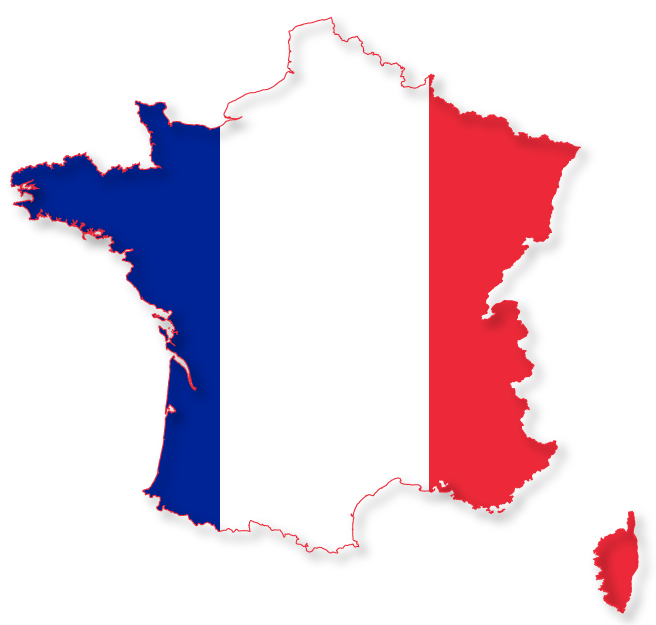
\includegraphics[height=2em]{img/france.png}}}{}}
%\addcontentsline{toc}{section}{\texorpdfstring{\protect\raisebox{-0.5ex}{\protect\makebox[3ex]{\protect
\includegraphics[height=1em]{img/flag-france.png}}}}{} in French}
%%% =============================================================
%%\index{Summary!en français}
%%\index{Summary!en français \protect\makebox[3ex]{\protect
\includegraphics[height=1em]{img/flag-france.png}}}
%\index{Summary!Résumé \protect\makebox[3ex]{\protect
\includegraphics[height=1em]{img/flag-france.png}}}
%
%Pour vous simplifier beaucoup de tâches longues et ardues, vous avez
%certainement déjà utilisé un ordinateur et en étiez très satisfaits.
%% 
%Cependant, de temps à autre, l'ordinateur ne fait pas ce que vous lui
%demandez: vous cliquez sur le bouton ``Faire ça'' et il ne le fait
%pas. Ou pire, l'ordinateur se bloque et ne répond plus à aucune
%commande. D'importantes heures de travail viennent peut-être de
%s'envoler.
%% 
%Vous gardez votre sang-froid, redémarrer l'ordinateur et tout semble à
%nouveau marcher comme prévu.
%% 
%L'erreur ne vient visiblement pas de l'ordinateur lui-même, mais elle
%semble venir du \emph{logiciel} qui contrôle ce dernier.
%% 
%Vous vous demandez pourquoi cette erreur n'a pas été corrigée, et qui
%plus est, pourquoi on ne s'est pas \emph{assuré} dès le départ que
%l'erreur ne survient pas. %survient
%
%Les différentes composantes électriques de la machine peuvent tomber
%en panne. Historiquement, ces erreurs sont appelées des \emph{bugs} %
%-- le terme anglais pour cafards -- %,
%car il est dit qu'un vrai cafard est entré un soir dans le châssis
%d'une machine qu'un informaticien fabriquait dans son garage,
%détruisant au passage quelques morceaux du circuit électrique. En se
%réveillant le lendemain, il s'est rendu compte que la machine
%manifestait un comportement bizarre.  Le terme est resté et est
%maintenant utilisé pour qualifier toutes sortes d'erreurs de
%programmation en général.
%% , c'est-à-dire quand un programme ne
%% solutionne pas le problème donné.
%
%Étant donné la complexité des ordinateurs de nos jours, il n'est pas
%étonnant qu'ils soient sujets à de nombreuses erreurs.
%% 
%Ils nécessitent de prendre en charge une multitude de
%paramètres, %et de caractéristiques,
%sans oublier les erreurs humaines introduites lors de la phase de
%programmation.
%% 
%C'est pourquoi %il est préférable
%la tendance est %
%de construire ces machines en composant plusieurs unités plus
%réduites.
%% 
%Chaque unité est de ce fait plus facile à contrôler, mais
%ces unités peuvent communiquer les unes avec les autres à n'importe
%quel moment.
%% 
%Il devient alors très difficile de prendre en compte tous les
%scénarios possibles et de prédire le comportement général du
%programme, à cause de ce caractère imprévisible. % hasardeux
%
%Les entreprises fabriquant ces logiciels n'ont pas intérêt à y laisser
%des bugs, puisqu'une erreur %quelque part
%peut engendrer d'autres erreurs en cascade.
%% 
%Celles-ci passent du temps, et de l'argent, à traquer ces bugs et s'il
%y en a trop, il n'est simplement plus rentable ou même envisageable de
%les éliminer.
%% 
%Les entreprises mettent donc en place, dans le cycle de développement de
%chaque projet, une phase essentielle de contrôle de qualité.
%% 
%Cela dit, certains bugs sont plus urgents à résoudre que d'autres.
%% 
%Ce n'est pas très grave si on ne peut pas décrocher son téléphone lors
%d'un appel, ou si l'éditeur de texte perd les derniers ajouts à notre
%document. C'est peut-être très ennuyeux mais le pronostic vital n'est
%pas engagé! On s'en remettra, en attendant la mise à jour du logiciel
%incriminé.
%% 
%Par contre, ce n
%'est pas le cas pour ces systèmes, dits
%\emph{critiques}, pour lesquels la sûreté est primordiale. Toutes les
%erreurs doivent être éliminées, qu'elles soient au niveau logiciel ou
%au niveau de la machine.
%% 
%Il n'est pas acceptable, par exemple, qu'un pacemaker s'arrête de
%fonctionner quand on passe le portique dans le métro, que l'avion
%parte en chute libre quand l'équipage allume le signal d'interdiction
%de fumer à bord, ou encore que deux trains entrent en collision parce
%que les feux ont mal fonctionné.
%% 
%% C'est pourquoi 
%Il est nécessaire de concevoir des techniques pour détecter ce genre
%d'erreurs.
%
%Pour améliorer la qualité des logiciels, il existe une technique
%prédominante: la méthode qui vise à soumettre le programme à une série
%de \emph{tests} et d'en observer les résultats.
%% 
%Ces scénarios de tests sont soigneusement conçus afin de couvrir un
%maximum d'exécution possible du programme.
%% 
%Dans la même catégorie, il est possible d'extraire un \emph{modèle} du
%programme %
%% , en prenant soin d'éliminer les morceaux superflus pour les
%% tests en cours, et 
%et de l'utiliser pour \emph{simuler} le programme.
%% 
%Cela dit, lorsque le programme est de plus en plus grand et complexe,
%que l'on utilise un modèle ou le programme lui-même, il devient
%impossible de \emph{garantir} que toutes les exécutions soient prises
%en compte par une batterie de scénarios.
%% 
%C'est même tout bonnement impossible lorsque le programme contient un
%paramètre qui varie sur un domaine non borné, comme par exemple, un
%entier.
%% 
%Ces deux méthodes sont utiles pour découvrir rapidement de simples
%erreurs, mais les erreurs subtiles, comme celles concernant le timing,
%restent non détectées.
%% 
%Dans le cas des systèmes qui requièrent une sûreté maxi\-male, il
%n'est pas concevable d'utiliser un programme qui pourrait contenir une
%erreur, quand bien même il ait passé tous ses tests.
%
%Comment donc s'assurer que toutes les exécutions d'un programme aient
%été prises en compte?
%% 
%On ne peut certainement pas faire tourner le programme et se contenter
%d'un ensemble restreint d'exécutions ou de valeurs pour les paramètres
%du programme.
%% 
%La technique d'\emph{analyse statique} offre une couverture complète
%d'un programme, sans l'exécuter. Elle inspecte toutes les exécutions
%\emph{faisables}, c'est-à-dire celles que le programme \emph{peut}
%effectuer et non celles qu'il \emph{va} effectuer.
%% 
%Le code source du programme y est sous la loupe, qu'il soit lisible
%par un humain ou seulement par une machine.
%% 
%Chaque combinaison est prise en compte ce qui rend cette méthode
%rapidement ingérable.
%% On pourrait être moins naïf, et se limiter à
%% certaines parties du code qui peuvent contenir les erreurs. Cependant,
%% déterminer leur emplacement est certainement aussi difficile que de
%% chercher les erreurs elles-même.
%% 
%% Il nous faut une autre méthode. %
%Cette thèse se concentre autour du problème suivant: %
%concevoir une méthode qui \emph{garantisse} qu'aucune erreur ne reste
%inaperçue, tout en restant dans des proportions raisonables.
%
%%% ------------------------
%Pour pouvoir vérifier qu'un programme soit correct, il s'agit d'abord
%de définir ce à quoi il doit se conformer ---appelé formellement sa
%\emph{spécification}.
%% 
%En listant l'ensemble des configurations à éviter, en listant tous les
%comportements souhaitables (ou une combinaison des deux), on décrit
%les propriétés que le programme doit satisfaire.
%% 
%Il en existe deux catégories: les propriétés de \emph{sûreté} et les
%propriétés de \emph{vivacité} (Safety et Liveness en anglais).
%% 
%Par exemple, ``le pacemaker ne s'arrête jamais'', ``l'airbag ne doit
%pas prendre plus de $x$~millisecondes pour s'ouvrir'', ou encore
%``aucun processus ne peut bloquer tous les autres'' sont des
%propriétés de sûreté. On doit s'assurer que le programme ne soit
%jamais dans une mauvaise configuration.
%% 
%À l'inverse, ``le facteur livre le courrier à son destinataire'', ``le
%système ne stagne pas'' ou encore ``le serveur prend en charge une
%requête internet'' sont des propriétés de vivacité, où l'on
%s'intéresse aux bonnes configurations du programme, associées à
%certaines probabilités.
%% 
%C'est à nous de définir ce que la spécification doit inclure, pour
%s'accorder avec la vérification souhaitée.
%% 
%Un système d'anti-blocage de freins (ABS), par exemple, calcule le
%freinage adéquate. Toutefois, si ce calcul ne se fait pas dans le
%temps imparti, le système n'est pas considéré comme un comportement
%désirable, et est donc défectueux.
%% 
%Dans cette thèse, nous nous concentrons sur les propriétés de sûreté.
%\begin{statement}
%  {\bf Sûreté}: %
%  {\it Étant donnée une spécification, le système peut-il se retrouver\\dans une mauvaise configuration?}
%\end{statement}
%
%%% ------------------------
%Plutôt que de tester le programme dans des scénarios particuliers, ou
%d'en analyser le code source, on utilise un cadre mathématique, dit de
%\emph{vérification formelle}, qui permette de \emph{prouver} qu'un
%programme soit conforme à sa spécification.
%% 
%Plus particulièrement, on cherche à prouver l'absence d'erreur, de
%manière \emph{automatique}, c'est-à-dire sans intervention de
%l'utilisateur.
%% 
%On commence par extraire un modèle qui corresponde aux comportements
%du programme origi\-nel, tout en en éliminant les parties sans
%rapport %importance
%au vu de la propriété à vérifier.
%% 
%Toutefois, comment faire lorsque le programme manipule des entités non
%bornées? On parle alors de système à états infinis et on en construit
%une approximation qui respecte malgré tout l'essence même du programme.
%
%De nombreux systèmes à états infinis peuvent en fait être caractérisés
%par une famille de systèmes à états finis, avec un paramètre (ou plus)
%variant dans un domaine non borné.
%% 
%Pour chaque valeur du paramètre, le système est à états finis.
%% 
%Le paramètre peut par exemple être 
%% la taille d'une base de données,
%le nombre de processus associés à une session donnée d'un protocole, %
%le nombre de n\oe{}uds dans les mailles d'un réseau, %
%ou encore l'agencement des différentes composantes d'un programme (et
%implicitement comment elles communiquent entre elles).
%% 
%Les systèmes qui contiennent un paramètre \emph{a priori} inconnu
%doivent se comporter correctement quelle que soit la valeur du
%paramètre. Ils sont ainsi considérés comme des systèmes à états
%infinis, et on les appelle des systèmes paramétrés.
%%
%%% ---------------------------
%Dans cette thèse, nous présentons deux méthodes pour vérifier certaines
%propriétés de sûreté de ces systèmes paramétrés.
% 
%La première méthode fait machine arrière: elle part des états erronés
%du système en général, et calcule à quoi ressembleraient les états du
%système qui pourraient mener à une erreur.
%% 
%Autrement dit, elle trouve l'ensemble des configurations qui sont
%directement et indirectement mauvaises.
%% 
%Si les états initiaux du système originel ne font pas partie de cet
%ensemble, le programme peut être considéré comme correct. Il faut bien
%sûr d'abord s'assurer que l'approximation du modèle extraite du
%programme de départ corresponde à ce dernier.
%
%La deuxième méthode démarre des états initiaux. Elle se limite à de
%petites valeurs du paramètre, et en déduit un seuil pour lequel il
%n'est pas nécessaire de continuer les calculs: la méthode a en effet
%toutes les données nécessaires pour conclure qu'il n'existe pas de
%mauvaises configurations pour les valeurs du paramètre plus grandes
%que ce seuil.
%% 
%En simplifiant, la méthode décompose chaque configuration en petits
%morceaux d'une certaine taille, et se charge de recombiner ces
%morceaux de toutes les manières possibles, en particulier en
%configurations de toutes tailles (un peu comme des briques de Lego).
%%
%L'idée est de collecter tous les petits morceaux, et de s'assurer
%qu'aucune des recombinaisons ne correspond à une mauvaise
%configuration.
%%
%Si c'est le cas, le seuil est trouvé. Si ce n'est pas le cas, on
%recommence avec des morceaux de taille un peu plus grande.
%
%En dernier lieu, il est intéressant de se demander dans quelles
%conditions la méthode termine. Le problème est classé dans la catégorie
%des problèmes indécidables, c'est-à-dire qu'il n'y a pas de méthode
%générale pour solutionner \emph{toutes} les instances du
%problème. Cela dit, pour certaines instances, ces deux méthodes
%s'avèrent être efficaces et peuvent même parfois être garanties de
%terminer.
%% 
%En effet, alors que d'autres méthodes prenaient des heures, ces
%méthodes permettent de vérifier certains programmes en quelques
%secondes, ce qui %Ces temps de calculs raisonnables étaient
%était le but recherché.
%%
%Cette thèse démontre notamment l'efficacité de ces méthodes en
%s'attaquant au problème complèxe d'analyse de formes, c'est-à-dire aux
%programmes concurrents manipulant des listes liées. %en mémoire.
%% \qed


\begingroup
\clearpage
% To adjust the indentation in your table of contents, uncomment and enter the widest numbers for each level
%  E.g.  \settocnumwidth{widest chapter number}{widest section number}{widest subsection number}...{...}
%  \settocnumwidth{5}{4}{5}{3}{3}{3}
%\initializepartialtoc
\tableofcontents
%\adjusttocfornonnumberedchapters % Adjusting the small ToC counters
\endgroup

%% Optional tables
%\listoftables
%\listoffigures

\chapter{How to read this thesis}
This document is a comprehensive summary.
\index{Thesis outline}

%\paragraph{Outline.}
\bigskip%
%
We first describe the domain of formal verification, where this thesis
belongs, and approach the problem in a top down fashion.

%
We present two techniques in
Chapter~\ref{chapter:monotonic:abstraction}~and~\ref{chapter:view:abstraction}
to prove safety properties for a wide range of programs (listed in
Chapter~\ref{chapter:case:studies}).
%
Finally, we dedicate Chapter~\ref{chapter:shape:analysis} to the
problem of shape analysis. It deals with a class of programs that
manipulate memory heaps concurrently.
%
To finish, we give some conclusions and potential directions for
future research topics.


\addtocontents{toc}{\protect\hrulefill}

%% -------------------------------------
 
%% -------------------------------------
\mainmatter
%% -------------------------------------


\input introduction
\input modelchecking
\input datastructure
\input correctness
\input shapeanalysis
\input conclusion

%\backmatter
%\addtocontents{toc}{\protect\hrulefill}
\addtocontents{toc}{\protect\mbox{}\protect\hrulefill\par}

%\chapter{Summaries of Papers}
\chapter{Summary of Contributions}

In this chapter, we give a short overview of our three peer-reviewed papers. We
will explain the problem addressed by each paper and its main contributions.
\		   

Automated verification of programs that manipulate complex dynamic linked data structures is a challenging problem in software verification. The problem becomes even more challenging when program correctness depends on relationships between data values that are stored in the dynamically allocated structures. 

In this paper, we present a general framework for verifying these programs. The underlying formalism of our framework is that
of forest automata (FA) which
has previously been developed for representing sets of reachable configurations of programs with complex dynamic linked data structures without data stored in nodes. In the FA framework, a heap
graph is represented as a composition of tree components. Sets of heap graphs can then
be represented by tuples of tree automata (TA). We extend FA by adding constraints between data elements associated with nodes of the heaps represented by FA, and we present extended versions of all operations needed for using the extended FA in a fully-automated verification approach, based on abstract interpretation.  
Technically, we express relationships between data elements associated with nodes of the heap graph by two classes of constraints. Local data constraints are associated with transitions of TA and capture relationships between data of neighbouring nodes in a heap graph; they
can be used, e.g., to represent ordering internal to some structure such as a binary search
tree. Global data constraints are associated with states of TA and capture relationships
between data in distant parts of the heap. In order to obtain a powerful analysis based on
such extended FA, the entire analysis machinery must have been redesigned, including
a need to develop mechanisms for propagating data constraints through FA, to develop a new inclusion check between
extended FAs, and to define extended abstract transformers

The resulting method allows for verification of pointer programs where the needed inductive invariants combine complex shape properties with constraints over stored data, such as sortedness. The method is fully automatic, quite general, and its efficiency is comparable with other state-of-theart analyses even though they handle less general classes of programs and/or are less automated. 







We have implemented our approach as an extension of the Forester tool and successfully applied it to a number of programs dealing with data structures such as various forms of singly- and doubly-linked lists, binary search trees, as well as skip lists. We presented experimental results from verifying programs dealing with variants of (ordered) lists and trees. To the best of our knowledge, our method is the first one to cope fully automatically with a full C implementation of a 3-level skip list. 

\section{Paper II: Automated Verification of Linearization Policies} 
Data structures that can be accessed concurrently by many parallel threads are a central component of many software applications, and are implemented in several widely used libraries (e.g., java.util.concurrent). Linearizabilityis the standard correctness criterion for such concurrent data structure implementations. It states that each operation on the data structure can be considered as being performed atom





rating operations announcing the occurrence of
LPs during each method invocation. The controller is occasionally activated, either by
its thread or by another controller, and mediates the interaction of the thread with the
observer as well as with other threads. Secondly, we handle the challenge of an unbounded number of threads by extending the successful thread-modular approach which verifies a concurrent program by generating an invariant that correlates the global state with the local state of an arbitrary thread. Finally,  we present a novel symbolic representation of singly-linked heap structures.
We have implemented our technique in a tool, and applied it to specify and automatically verify linearizability of all the implementations of concurrent set, queue,
and stack algorithms known to us in the literature, as well as some algorithms for implementing atomic memory read/write operations. To use the tool, the user needs to
provide the code of the algorithm together with the controllers that specify linearization
policies. To our knowledge, this is the first time all these examples are verified fully
automatically in the same framework.
\section{Paper III: Fragment Abstraction for Concurrent Shape Analysis}  
A major challenge in automated verification is to develop techniques
that are able to reason about fine-grained concurrent algorithms that consist of
an unbounded number of concurrent threads, which operate on an unbounded
domain of data values, and use unbounded dynamically allocated memory. Existing automated techniques consider the case where shared data is organized into
singly-linked lists.

In this paper, we present a technique for automatic verification of concurrent data structure implementations that operate on dynamically allocated heap structures which are more complex than just singly-linked lists. Our approach is the first
framework that can automatically verify concurrent data structure implementations that
employ singly linked lists, skiplists [15, 23, 39], as well as arrays of singly linked
lists [11], at the same time as handling an unbounded number of concurrent threads,
an unbounded domain of data values (including timestamps), and an unbounded shared
heap.

Our technique is based on a novel shape abstraction, called fragment abstraction,
which in a simple and uniform way is able to represent several different classes of
unbounded heap structures. Its main idea is to represent a set of heap states by a set
of fragments. A fragment represents two heap cells that are connected by a pointer
field. For each of its cells, the fragment represents the contents of its non-pointer fields,
together with information about how the cell can be reached from the program’s pointer
variables. The latter information consists of both: (i) local information, saying which
pointer variables point directly to them, and (ii) global information, saying how the cell
can reach to and be reached from (by following chains of pointers) other heap cells that
are significant from a global perspective, typically since they are pointed to by global
variables. A set of fragments represents the set of heap states in which any two pointerconnected nodes is represented by some fragment in the set. Thus, a set of fragments
describes the set of heaps that can be formed by “pieced together” fragments in the
set. The combination of local and global information in fragments supports precise
reasoning about the sequence of cells that can be accessed by threads that traverse the
heap by following pointer fields in cells and pointer variables: the local information
captures properties of the cell fields that can be accessed as a thread dereferences a
pointer variable or a pointer field; the global information also captures whether certain
significant accesses will at all be possible by following a sequence of pointer fields. This
support for reasoning about patterns of cell accesses enables automated verification of
reachability and other functional properties.
Fragment abstraction can (and should) be combined, in a natural way, with data abstractions for handling unbounded data domains and with thread abstractions for handling an unbounded number of threads. For the latter we adapt the successful threadmodular approach [5], which represents the local state of a single, but arbitrary thread,
together with the part of the global state and heap that is accessible to that thread. Our
combination of fragment abstraction, thread abstraction, and data abstraction results in
a finite abstract domain, thereby guaranteeing termination of our analysis.
We have implemented our approach and applied it to automatically verify correctness, in the sense of linearizability, of a large number of concurrent data structure
algorithms, described in a C-like language. More specifically, we have automatically
verified linearizability of most linearizable concurrent implementations of sets, stacks,
and queues, and priority queues, which emply singly-linked lists, skiplists, or arrays
of timestamped singly-linked lists, which are known to us in the literature on concurrent data structures. For this verification, we specify linearizability using the simple and
powerful technique of observers [1, 7, 21, 3], which reduces the criterion of linearizability to a simple reachability property. To verify implementations of stacks and queues,
the application of observers can be done completely automatically without any manual
steps, whereas for implementations of sets, the verification relies on light-weight user
annotation of how linearization points are placed in each method. 

\section{Related Work}
This chapter reviews related work, along the main topics of this thesis including: verification of linearizabilities of concurrent algorithms, 
sequential shape analysis and concurrent techniques.
\subsection{Linearizabilities}
Much previous work has been devoted to
the {\it manual} verification of linearizability for
concurrent programs such as \cite{Aaron:locigcal:linearizability}.
In \cite{OHearnlist}, O'Hearn {\it et al.}  define a
{\it hindsight lemma} that
provides a non-constructive evidence for linearizability. 
%
The lemma is used to prove linearizability of an optimistic variant of 
the lazy set algorithm.
%% by identifying the hindsight property of the algorithm. 
Vafeiadis \cite{Vafeiadis:Thesis}
uses forward and backward simulation relations together
with history or prophecy variables to prove linearizability.
%
These approaches are manual, and without
tool implementations.
{\it Mechanical} proofs of linearizability, using interactive theorem
provers, have been reported in 
\cite{Colvin:Lazy-List,Derrick:fm14,SWD:cav12,SDW:tcl14}.
%
For instance, Colvin {\it et al.} \cite{Colvin:Lazy-List}
verify the lazy set algorithm in  PVS,
using a combination of forward and backward simulations.

There are several works on {\it automatic} verification of linearizability.
%
In \cite{Vafeiadis:cav10}, Vafeiadis
develops an automatic tool for proving  linearizability that
employs instrumentation to verify logically pure executions.
%
However, this work can handle non-fixed LPs only for read-only methods,
i.e, methods that do not modify the heap.
%
This means that the method cannot handle
 algorithms like the {\it Elimination} queue ~\cite{Shavit:ElimQueue}, {\it HSY} stack~\cite{HSYstack}, {\it CCAS}~\cite{Harris:CAS}, 
{\it RDCSS}~\cite{Harris:CAS} and {\it HM} set~\cite{ArtOfMpP} that we consider in this paper. In addition, their shape abstraction is not powerful enough to handle algorithms like {\it Harris} set~\cite{Harris:list} and {\it Michael} set~\cite{Michael:list} that are also handled by our method.
%
%For instance, in the {\it HSY} stack algorithm both
%the {\tt push} and {\tt pop} operations modify
%the heap and help each other~\cite{HSYstack}. 
%
Chakraborty {\it et al.} \cite{HSV:concur13}
describe an ``aspect-oriented'' method for  modular verification 
of concurrent queues that they use to prove linearizability of the Herlihy/Wing queue.
Bouajjani et al. \cite{BEEH:icalp15} extended this work to show that verifying 
linearizability for certain
fixed abstract data types, including queues and stacks, is reducible to 
control-state reachability. 
%
We can incorporate this technique into
our framework by a suitable construction of observers.
The method can not be applied to sets.
%
The most recent work of Zhu {\it et al.} \cite{Poling}
describe a tool that is applied for specific set, queue, and stack  
algorithms. For queue algorithms, their technique can handle queues with helping mechanism except for {\it HW} queue~\cite{HeWi:linearizability} which is handled by our paper.
%
For set algorithms, the authors can only handle those that perform an optimistic contains (or lookup) operation by applying the {\it hindsight lemma} from 
\cite{OHearnlist}. 
%
Hindsight-based proofs provide only {\it non-constructive} 
evidence of linearizability. Algorithms with non-optimistic contains (or lookup) operation like {\it HM}~\cite{ArtOfMpP}, {\it Harris}~\cite{Harris:list} and {\it Michael}~\cite{Michael:list} sets cannot be verified by their technique.  
%
Vechev {\it et al.}~\cite{Vechev:spin09}
check linearizability with user-specified non-fixed LPs,
using a tool for finite-state verification.
Their method assumes a bounded number of threads, and
they report state space explosion when having more than two threads.
%
Dragoi  {\it et al.} \cite{Henzinger:CAV13} describe a method for proving
linearizability that is applicable to algorithms with non-fixed LPs.
%
However, their method needs to rewrite the implementation so that all operations 
have linearization points within the rewritten code.
%
\v{C}ern{\'y} {\it et al} \cite{CernyRZCA:CAV10} show decidability of a class
of programs with a bounded number of threads operating on concurrent data structures.
%
%% This paper is about a different problem
%% Horn and Kroening \cite{Kroening-Linearizability:FORTE15}
%% have recently presented an efficient linearizability checker based on {\it P-compositionality} 
%% which can be applied when having a bounded number of threads.
%
Finally, the works~\cite{AHHR:integrated,BLMRS:cav08,Vafeiadis:vmcai09}
all require fixed linearization points.

We have not found any report in the literature of a
verification method that is sufficiently powerful to
automatically verify the class of concurrent set
implementations based on sorted and non-sorted
singly-linked lists having non-optimistic contains (or lookup) operations we consider. For instance %For instance,
%the shape abstraction of the CAVE implementation
%\cite{Vafeiadis:cav10}
%is not powerful enough to handle
the lock-free sets of {\it HM}~\cite{ArtOfMpP},
{\it Harris}~\cite{Harris:list}, or {\it Michael}~\cite{Michael:list},
or unordered set of~\cite{Zhang:unorderedlist},
%reported in
%Section~\ref{section:experiments} (as also confirmed by the CAVE
%tool implementors).
%The same applies to
%the tool in~\cite{Poling}.


\subsection{Shape Analysis}
\subsubsection{Sequential Shape Analysis}
Our approach builds on the fully automated FA-based
approach for shape analysis of programs with complex dynamic linked data
structures \cite{forester11,boxes13}. We significantly extend this approach by
allowing it to track ordering relations between data values stored inside
dynamic linked data structures. 

For shape analysis, many other formalisms than FA have been used, including,
e.g., separation logic and various related graph formalisms
\cite{InvaderCAV08,thor10,rival11,dudka13}, other logics \cite{Sagiv02,pale97},
automata \cite{artmc12}, or graph grammars \cite{juggrnaut10}. Compared with FA,
these approaches typically handle less general heap structures (often restricted
to various classes of lists) \cite{InvaderCAV08,dudka13}, they are less
automated (requiring the user to specify loop invariants or at least inductive
definitions of the involved data structures)
\cite{thor10,rival11,dudka13,juggrnaut10}, or less scalable \cite{artmc12}.

Verification of properties depending on the ordering of data stored in SLLs was
considered in~\cite{lists-counters}, which translates programs with SLLs to
counter automata. A subsequent analysis of these automata allows one to prove
memory safety, sortedness, and termination for the original programs. The work
is, however, strongly limited to SLLs. In this paper, we get inspired by the way
that \cite{lists-counters} uses for dealing with ordering relations on data, but
we significantly redesign it to be able to track not only ordering between
simple list segments but rather general heap shapes described by FA. In order to
achieve this, we had to not only propose a suitable way of combining ordering
relations with FA, but we also had to significantly modify many of the
operations used over FA.

In~\cite{atva09}, another approach for verifying data-dependent properties of
programs with lists was proposed. However, even this approach is strongly
limited to SLLs, and it is also much less efficient than our current approach.
In~\cite{haziza:tacas13}, concurrent programs operating on SLLs are analyzed
using an adaptation of a transitive closure logic~\cite{BiRa:vmcai06}, which
also tracks simple sortedness properties between data elements.

Verification of properties of programs depending on the data stored in dynamic
linked data structures was considered in the context of the TVLA tool
\cite{Loginov:AbstrRefViaInductLearning:05} as well. Unlike our approach,
\cite{Loginov:AbstrRefViaInductLearning:05} assumes a fixed set of shape
predicates and uses inductive logic programming to learn predicates needed for
tracking non-pointer data. The experiments presented in
\cite{Loginov:AbstrRefViaInductLearning:05} involve verification of sorting and
stability properties of several programs on SLLs (merging, reversal,
bubble-sort, insert-sort) as well as insertion and deletion in BSTs. We do not
handle stability, but for the other properties, our approach is much faster.
Moreover, for BSTs, we verify that a node is greater/smaller than all the nodes
in its left/right subtrees (not just than the immediate successors as in
\cite{Loginov:AbstrRefViaInductLearning:05}).

An approach based on separation logic extended with constraints on the data
stored inside dynamic linked data structures and capable of handling size,
ordering, as well as bag properties was presented in \cite{sleek12}. Using the
approach, various programs with SLLs, DLLs, and also AVL trees and red-black
trees were verified. The approach, however, requires the user to manually
provide inductive shape predicates as well as loop invariants.  Later, the need
to provide loop invariants was avoided in \cite{sleek13}, but a need to manually
provide inductive shape predicates remains.

Another work that targets verification of programs with dynamic linked data
structures, including properties depending on the data stored in them, is
\cite{Zee:pldi08}. It generates verification conditions in an undecidable
fragment of higher-order logic and discharges them using decision procedures,
first-order theorem proving, and interactive theorem proving. To generate the
verification conditions, loop invariants are needed. These can either be
provided manually or sometimes synthesized semi-automatically using the approach
of \cite{wies07hav}. The latter approach was successfully applied to several
programs with SLLs, DLLs, trees, trees with parent pointers, and 2-level skip
lists. However, for some of them, the user still had to provide some of the
needed abstraction predicates.
Several works, including~\cite{dragoi:atva12}, define frameworks for reasoning
about pre- and post-conditions of programs with SLLs and data. Decidable
fragments, which can express more complex properties on data than we consider,
are identified, but the approach does not perform fully automated verification,
only checking of pre-post condition pairs.
\subsubsection{Concurrent Shape Analysis}
A large number of techniques have been developed for representing heap structures
in automated analysis, including,
e.g., separation logic and various related graph formalisms
\cite{InvaderCAV08,rival11,dudka13}, other logics \cite{SRW:threevalued},
automata \cite{boxes13}, or graph grammars \cite{juggrnaut10}. 
Most works apply these to sequential programs.

Approaches for automated verification of concurrent algorithms are limited to the
case of singly-linked
lists~\cite{AHHR:integrated:short,meyer:vmcai16,Quy:sas16,Sagiv:correlation,Vafeiadis:cav10}.
Furthermore, many of these techniques impose additional restrictions on the considered verification problem, such as bounding the number of accessing
threads~\cite{Amit:comparisonAbstraction,Vechev:spin09,CernyRZCA:CAV10}.

In~\cite{AHHR:integrated:short}, concurrent programs operating on SLLs are analyzed
using an adaptation of a transitive closure logic~\cite{BiRa:vmcai06}, combined with
tracking of simple sortedness properties between data elements; the approach does
not allow to represent patterns observed by threads when following sequences of
pointers inside the heap, and so has not been applied to concurrent set
implementations.
In our recent work~\cite{Quy:sas16}, we extended this approach to handle SLL implementations
of concurrent sets by adapting a
well-known abstraction of singly-linked lists ~\cite{MYRS:Canonical} for concurrent programs.
The resulting technique is specifically tailored for singly-links.
Our fragment abstraction is significantly simpler conceptually, and can therefore be  adapted
also for other classes of heap structures.
The approach of~\cite{Quy:sas16} is the only one with a shape representation strong enough to
verify  concurrent set
implementations based on sorted and non-sorted
singly-linked lists having non-optimistic contains (or lookup) operations we consider, such as
the lock-free sets of {\it HM}~\cite{ArtOfMpP},
{\it Harris}~\cite{Harris:list}, or {\it Michael}~\cite{Michael:list},
or unordered set of~\cite{Zhang:unorderedlist}. As shown in
Section~\ref{section:experiments}, our fragment abstraction can handle them
as well as also algorithms employing skiplists and arrays of singly-linked lists.

There is no previous work on automated verification of skiplist-based concurrent algorithms.
Verification of {\em  sequential} algorithms have been addressed under restrictions, such as limiting the
number of levels to two or three~\cite{boxes13,Quy:atva13:journal}. The work~\cite{Sanchez:skiplists}
generates verification conditions for statements in sequential skiplist implementations. All these
works assume that skiplists have the well-formedness property that any higher-level lists is a
sublist of any lower-level list, which is true for sequential skiplist algorithms, but false for
several concurrent ones, such as~\cite{ArtOfMpP,Linden:opodis13}.



Concurrent algorithms based on arrays of SLLs, and including timestamps, e.g.,
for verifying the algorithms in~\cite{ts-stack} have shown to be rather challenging. Only
recently has the TS stack been verified by non-automated
techniques~\cite{BEEM:cav17} using a non-trivial extension of
forward simulation, and the TS queue been verified manually by a new technique
based on partial orders~\cite{Khyzha:esop17,singh:issre16}..
We have verified both these algorithms automatically using fragment abstraction,

Our fragment abstraction is related in spirit to other formalisms that
abstract dynamic graph structures by defining some form of equivalence on
its nodes (e.g.,~\cite{spotlight07,SRW:threevalued,boxes13}). These have
been applied to verify functional correctness fine-grained concurrent
algorithms for a limited number of SLL-based algorithms. Fragment
abstraction's representation of both local and global information allows to
extend the applicability of this class of techniques.
%\newcommand{\contribitem}[1]{\tikz[baseline=(c.base)]\node(c)[paper]{\ref{paper:#1}};}
%
%\noindent%\vspace{1\baselineskip}%
%\begin{list}{%
%    Hey% Cheating
%  }{%
%    \raggedright%
%    \setlength{\leftmargin}{2,5em}%
%    \setlength{\labelsep}{1em}%
%    \setlength{\itemsep}{1em plus 0.2em minus 0.2em}%
%    \setlength{\parsep}{0mm}%
%    \setlength{\topsep}{0mm}}%
%
%\item[\contribitem{ATVA13}] %
%  I designed the method with \lukas. %
%  I am the sole implementer of the prototype and responsible for the experimentation. %
%  I participated in all parts of the writing, equally as my co-authors. %
%
%\item[\contribitem{SAS16}] %
%  I designed the method with \lukas\ and \ahmed. %
%  I am the sole implementer of the prototype and responsible for the experimentation. %
%  I participated in all parts of the writing, equally as my co-authors. %
%
%\item[\contribitem{SAS14}] %
%  I designed the method with \lukas. %
%  I am the sole implementer of the prototype and responsible for the experimentation. %
%  I participated in all parts of the writing, equally as my co-authors. %
%
%\end{list}\nopagebreak%

\chapter{Conclusion and Future Work}
\label{chapter:conclusion}
\label{chapter:future:work}
%\paragraph{Conclusion} 
We have presented, in this thesis, approaches to verify the complex problem of
both sequential and concurrent heap manipulating programs.%
Such programs induce an infinite-state space in several dimensions:
they %
(i) consist of an unbounded number of concurrent threads, %
(ii) use unbounded dynamically allocated memory, and %
(iii) the domain of data values is unbounded. %
(iv) consist of un unbounded number of pointers. In addition, the linearization points of some programs are not fixed. They are depended on the future executions of these programs. In this thesis, we focus on proving both safety properties, and linearization properties for the system, regardless of the value of this parameter. In order to prove safety properties, we defines an abstract model of the program, and we employ approximation techniques to that ignore irrelevant information so that we can reduce the problem
into a finite-state model. In fact, we use an over-approximation, such that the abstract model
cover all the behaviors of the original system. However, it might cover other behaviors which are not in the original system. If the bad states are not reached during the computation of reachable states of the abstract model, then the abstract model is considered safe, and so is the original system is also safe. If the bad state is reachble, we have to refine the abstraction. In order to verity linearization properties of a program, we add a specification which expresses its a data structure, using the technique of observers. In our approaches, the user have to provide linearization policies which specify how the program is linearized. We use a technique call {\tt controller} to specify linearization policies. We then verify that in any concurrent execution of a collection of method calls, the sequence of announced operations satisfies the semantics of the data structure. This check is performed by an observer, which monitors the sequence of announced operations. This reduces the problem of checking linearizability to the problem of checking that in this cross-product, the observer cannot reach a state where the semantics of the set data structure has been violated. To verify that that the observer cannot reach a state where a violation is reported, we compute a symbolic representation of an invariant that is satisfied by all reachable configuration of the cross-product of a program and an observer.%of an invariant that is satised by all reachable configurations of the cross-product of a program and an observer


%\paragraph{Future work} 
There are two main possible lines of future work we would like to work on from this thesis. The first line is to
extend the type programs we consider, by allowing more complicated data structures such as trees and design methods that allow the automatic synthesis of the controllers. Another possible line of work is to extend the view abstraction to
multi-threaded programs running on machines with different memory
models. Such hardware systems employ store buffers and cache systems
that could be modeled using views. This is an interesting challenge since it would help programmers to
write their code under a given memory model that is simpler to reason
around, and verify that the behaviour of the program is the same under
another less-restricted memory model.





%\addtocontents{toc}{References}
% No restriction is set to the reference styles
\nocite{*} % Remove this for your own citations
\bibliographystyle{plain}
%\bibliographystyle{alpha}
\bibliography{misc/references}

%% Index %%%%%%%%%%%%%%%%%%%%%%%%%%%%%%%
\ifnoindex\else
% \phantomsection
% \addcontentsline{toc}{chapter}{\indexname}
\printindex
\fi
%%%%%%%%%%%%%%%%%%%%%%%%%%%%%%%%%%%%%%%%

%% -------------------------------------

%%%%%%%%%%%%%%%%%%%%%%%%%%%%%%%%%%%%%%%%%%%
\end{document}
%%%%%%%%%%%%%%%%%%%%%%%%%%%%%%%%%%%%%%%%%%%
